\begin{SingleSpace}
\chapter{Equilibrium Zonal Flow in the Atmospheres of Tidally Locked Planets}\label{ch:eqm-zonal-flow}
\vspace{0.5cm}
\chapterprecishere{``One might as well approximate the derivatives well instead of badly''\par\raggedleft--- \textup{John P. Boyd}, Chebyshev and Fourier Spectral Methods}
\end{SingleSpace}
\vspace{0.5cm}

%0 -- LEAD-IN PARAGRAPHS

This thesis aims to understand the global circulation of tidally locked planets. The natural place to start is with their dominant dynamical component -- the flow from day-side to night-side. This sets observable quantities such as the  temperature of both sides and the position of the hot-spot \citep{pierrehumbert2018review}. It also dominates the transport of condensable species and clouds with consequences for climate stability and habitability \citep{ding2016convection} \citep{pierrehumbert2016dynamics} \citep{komacek2019atmospheric}.

%FRAMING TEXT

This flow from day-side to night-side would be isotropic in all directions away from the substellar point on a non-rotating planet. On any real planet, the Coriolis force modifies this flow, giving an asymmetric flow that is eastward at the equator in most cases \citep{showman2011superrotation}. Eastward flow at the equator is ``superrotating'' by definition \citep{read2018superrotation}, so this zonal flow is often referred to offhand as an ``equatorial superrotating jet''.

%SIGNPOSTS

In this chapter, I will discuss the formation and equilibration of this flow. I will review \citet{showman2010superrotation} and \citet{showman2011superrotation}, which set out the current understanding of superrotation at the equator. I will then introduce a modification to their shallow-water model, which we found necessary to resolve a difference between this model and GCM simulations. I will show how this modification let us qualitatively understand the formation of different zonal flow profiles in tidally locked planetary atmospheres.

%SUMMARISE CONCLUSIONSß

I will conclude that the zonal flow profile is a subtle but important part of the atmosphere of these planets. This will  lead directly into Chapter \ref{ch:wave-mean-flow}, which shows the effect of the zonal flow profile on the temperature distribution of these atmospheres, which governs the observable thermal radiation from these planets.

%START ELEMENT

%%%%%%%%%%%%%%%%%%%%%%%%%%%%%%%%%%%%
%SECTION 1 -- LINEAR SHALLOW-WATER AND UNIFORM FLOW
\section{The Shallow-Water Equations}\label{sec:shallow-water}

We used the linear shallow-water equations on a one-layer equatorial beta-plane to model the atmosphere of a tidally locked planet. These equations describe the motion of a single layer of fluid of constant density where the horizontal scale of its flow is much greater than the depth of the fluid. The linear form of these equations describe small perturbations to this layer \citep{vallis2006book}. We model the atmosphere of a tidally locked planet with a similar shallow-water model to \citet{showman2011superrotation}. The model corresponds to an active upper layer following the single-layer shallow water equations, above a quiescent layer which can transport mass and momentum to and from the upper layer. The forcing due to stellar heating is represented by $Q$, a relaxation to the radiative equilibrium height field.

%SUBSECTION -- LINEAR SHALLOW-WATER
\subsection{Free Solutions}

In this section, we derive the wave response to stationary forcing on the beta-plane \citep{matsuno1966quasi}. The beta-plane system approximates the Coriolis parameter as linear, which is only accurate at low latitudes but leads to more intuitive and useful solutions than the full spherical geometry. We solve the equations in a spherical geometry in Section \ref{sec:sphere-solutions}, and show that the beta-plane approximation leads to very similar solutions, as in other studies of the atmospheres of tidally locked planets \citep{showman2011superrotation} \citep{heng2014analytical}.

All the quantities are linearized as the sum of a zonally mean background value $F(y)$  and a perturbation with the form  $f(y) e^{i( k_{x} x-\omega t)}$ (unlike \citet{matsuno1966quasi}, who uses the less conventional form  $f(y) e^{i( k_{x} x+\omega t)}$). Throughout this paper, we will use capital letters for mean zonal quantities such as $\bar{U}$ and $\bar{H}$, and lower-case letters for perturbations to this background, such as $u$ and $h$ (unless otherwise specified, such as the forcing $Q$). The shallow-water equations for these perturbations with zero background flow are:

\begin{equation}\label{eqn:sw-eqns-1}
  \begin{gathered}
     \frac{\partial u}{\partial t} - \beta y v +\frac{\partial h}{\partial x} = 0 \\
      \frac{\partial v}{\partial t} + \beta y u + \frac{\partial h}{\partial y} = 0 \\
    \frac{\partial h}{\partial t} +c^{2}(\frac{\partial u}{\partial x} + \frac{\partial v}{\partial y}) = Q(x,y) \\
  \end{gathered}
\end{equation}

where $h$ is the height, $c = \sqrt{gH}$ is the gravity wave speed \citep{matsuno1966quasi}, and there is no friction or damping. Non-dimensionalizing with time scale $\sqrt{1/c \beta}$ and length scale $\sqrt{c/\beta}$ (the equatorial Rossby radius of deformation $L_{R}$), and assuming all quantities have the form $f(y) e^{i( k x-\omega t)}$, the free equations with zero forcing are:

\begin{equation}\label{eqn:sw-eqns-2}
  \begin{gathered}
      - i \omega u - y v + i k_{x} h = 0 \\
      - i \omega v + y u + \frac{\partial h}{\partial y} = 0 \\
      - i \omega h + i k u + \frac{\partial v}{\partial y} = 0 \\
  \end{gathered}
\end{equation}

\citet{matsuno1966quasi} gives the free modes of this system as XX. Figure \ref{fig:free-kelvin-mode} shows the free Kelvin mode with wavenumber 1 and Figure \ref{fig:free-rossby-mode} shows the free Rossby mode with wavenumber 1. The eigenvalues of these modes will prove to be very important, as they set the longitudinal position of each mode in the response to forcing, which will produce the hot-spot shift in Section \ref{ch:wave-mean-flow}.

\begin{figure}
  \centering
  \begin{subfigure}[b]{0.49\textwidth}
    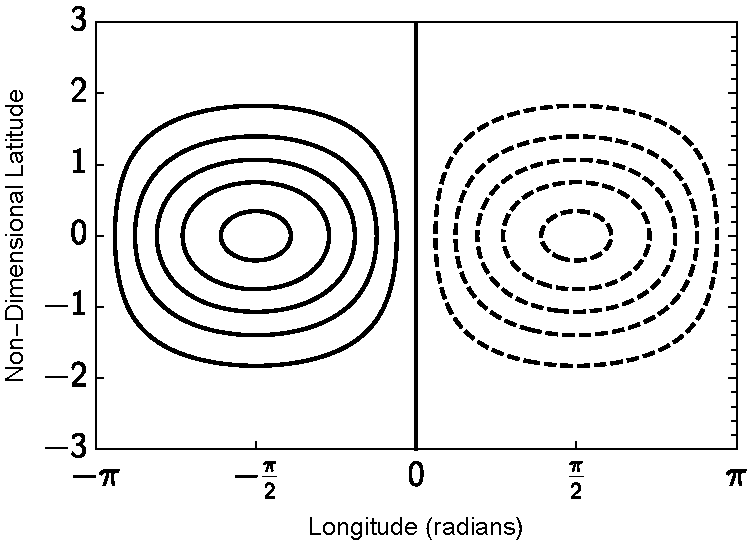
\includegraphics[width=1.0\textwidth]{figures/wave-mean-flow/free-kelvin-mode.pdf}
    \caption{Free Kelvin Mode.}
    \label{fig:free-kelvin-mode}
  \end{subfigure}
  %
  \begin{subfigure}[b]{0.49\textwidth}
    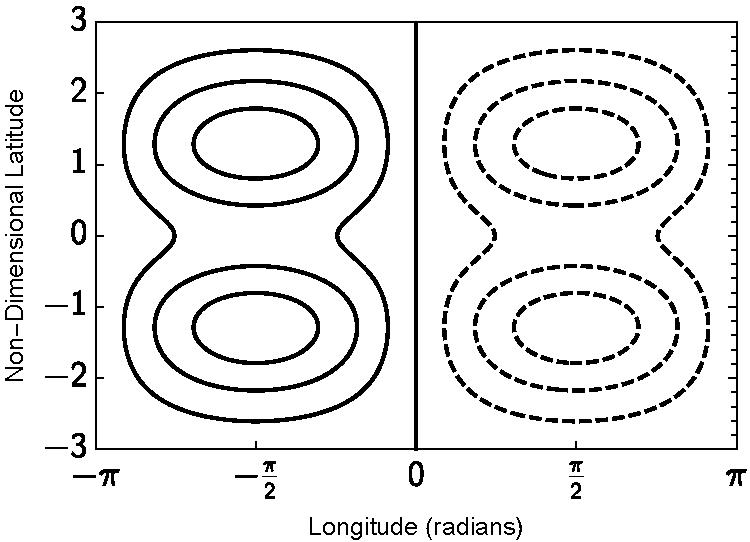
\includegraphics[width=1.0\textwidth]{figures/wave-mean-flow/free-rossby-mode.pdf}
    \caption{Free Rossby Mode.}
    \label{fig:free-rossby-mode}
  \end{subfigure}
  \caption{Free Modes.}
  \label{fig:free-kelvin-rossby-mode}
\end{figure}


%SUBSECTION --
\subsection{Forced Solutions}

In this chapter, I will focus on the response of the shallow-water equations to a forcing $Q(x,y)$ on the height field $h$, representing the stellar forcing on a tidally locked planet. The forced solution can be considered to be a sum of the free modes discussed in the previous section, at different locations and with different strengths.

The forced equations are:

\begin{equation}\label{eqn:sw-eqns-forced}
  \begin{gathered}
    \alpha_{dyn} u - \beta y v +\frac{\partial h}{\partial x} = 0 \\
    \alpha_{dyn} v + \beta y u + \frac{\partial h}{\partial y} = 0 \\
    \alpha_{rad} h + c^{2}(\frac{\partial u}{\partial x} + \frac{\partial v}{\partial y}) = Q(x,y) \\
  \end{gathered}
\end{equation}

with boundary conditions

\begin{equation}
  u , v , h \rightarrow 0 \quad \mathrm{for} \quad y \rightarrow \pm \infty.
\end{equation}

\citet{matsuno1966quasi} shows how the response of Equation \ref{eqn:sw-eqns-forced} to a forcing $Q(x,y) = Q_{0} \sin(x) e^{-y^{2}/2}$ and uniform damping $\alpha_{rad}=\alpha_{dyn}=\alpha$ can be found analytically as a sum of the free modes of the system. The forced response $\chi = (u,v,h)$ is a sum of the free modes $\xi_{m}=(u_{m},v_{m},h_{m})$, weighted by coefficients $a_{m}$

\begin{equation}
  \chi = \sum a _ { m } \xi _ { m },
\end{equation}

where the coefficients are given by

\begin{equation}
  a _ { m } = \frac { 1 } { \alpha - i \omega _ { m } } b _ { m },
\end{equation}

where $\omega_{m}$ is the eigenvalue of the mode $m$, and

\begin{equation}
  b _ { m } = \left[ \int \overline { \xi } _ { m } ( y ) \sigma ( y ) d y \right] / \left[ \int \left| \xi _ { m } ( y ) \right| ^ { 2 } d y \right].
\end{equation}

For the forcing $Q(x,y) = Q_{0} \sin(x) e^{-y^{2}/2}$, all of the coefficients $a_{m}$ are zero, apart from those for the Kelvin wave and the $n=1$ Rossby wave. Figure \ref{fig:motivate-showman} shows this forced response.

DO THIS! The eigenvalues determine the position of each free mode in the forced response.

In the rest of this chapter, I willl instead use the pseudo-spectral method described in Appendix \ref{ap:ps-methods} to find the response to forcing. This method works for any forcing and background flow (unlike the analytic method), and still finds the exact analytic solution for this case with zero background flow. Figure \ref{fig:motivate-showman} was actually calculated using this pseudo-spectral method rather than expanding in terms of the free modes, but the solution is identical (as explained in Appendix \ref{ap:ps-methods}, the basis functions of the pseudo-spectral method can exactly represent the free modes of the shallow-water system).

\begin{figure}
  \centering
  \begin{subfigure}[b]{0.49\textwidth}
    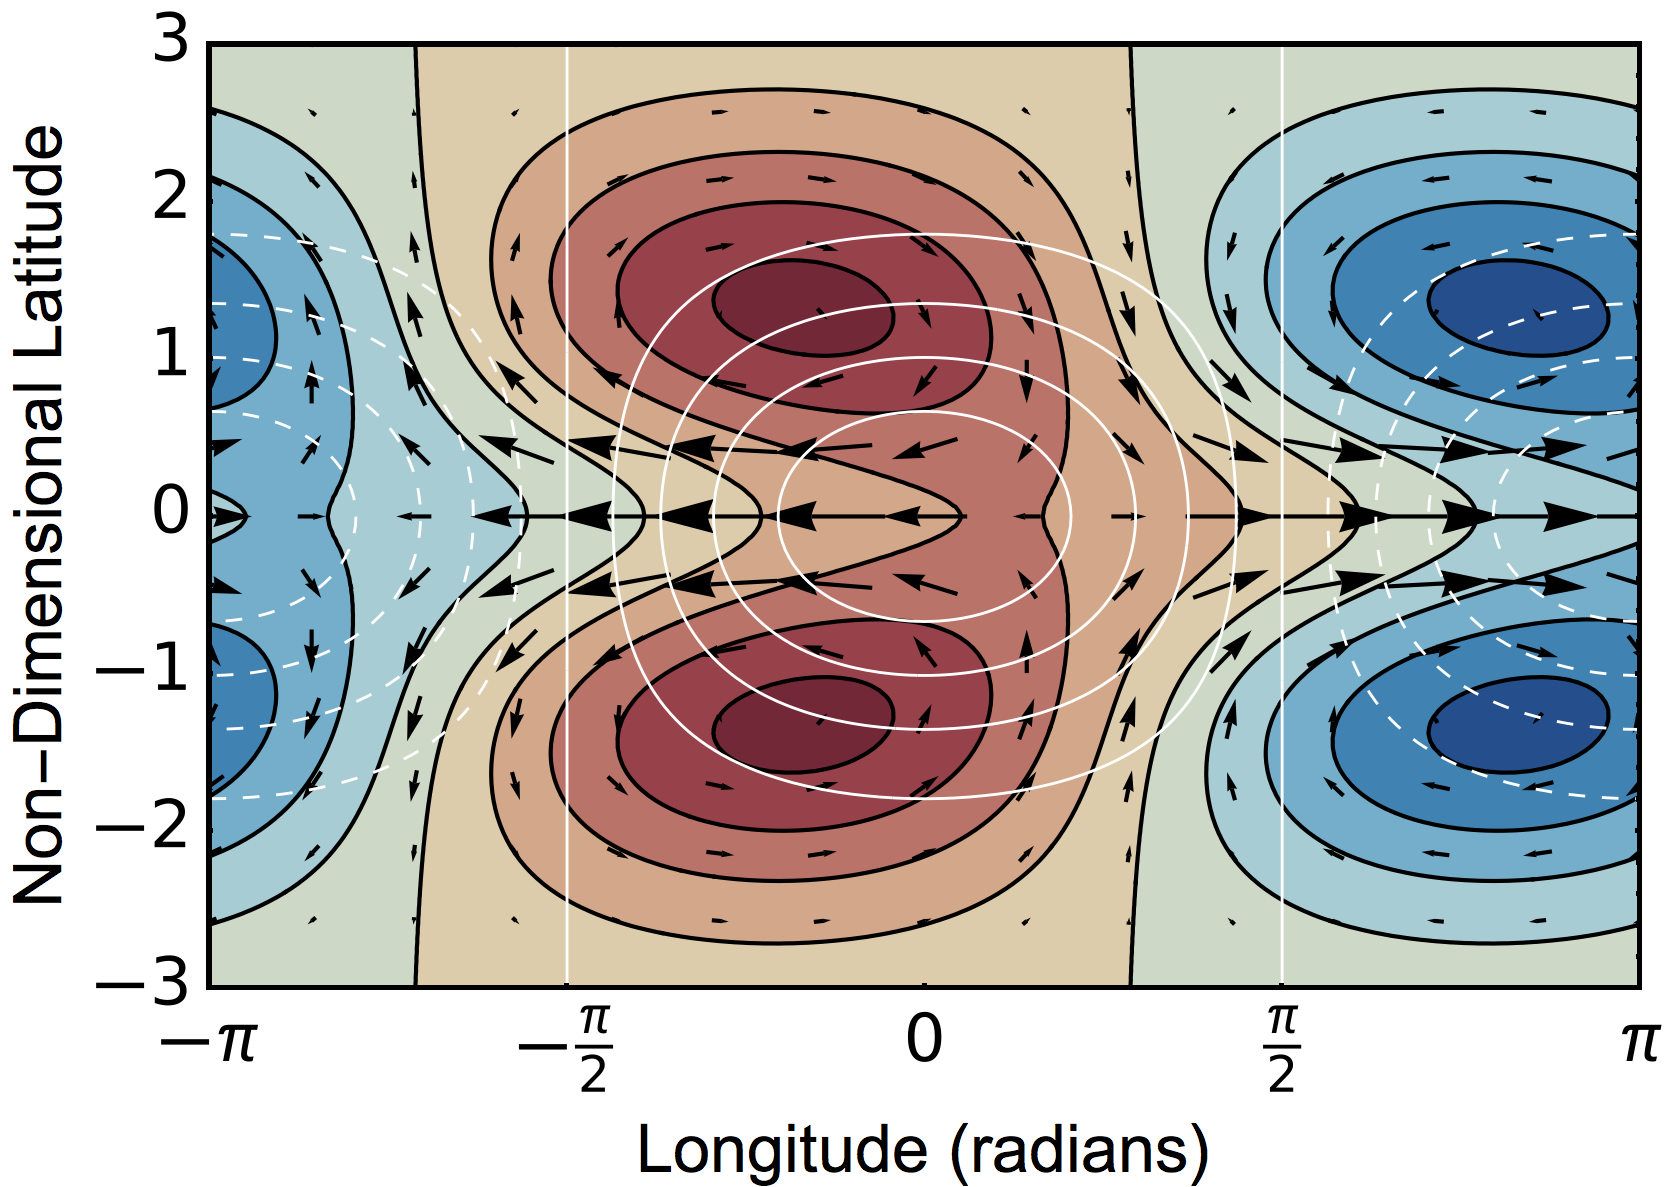
\includegraphics[width=1.0\textwidth]{figures/wave-mean-flow/motivate-showman.png}
    \caption{motivate-showman.}
    \label{fig:motivate-showman}
  \end{subfigure}
  %
  \begin{subfigure}[b]{0.49\textwidth}
    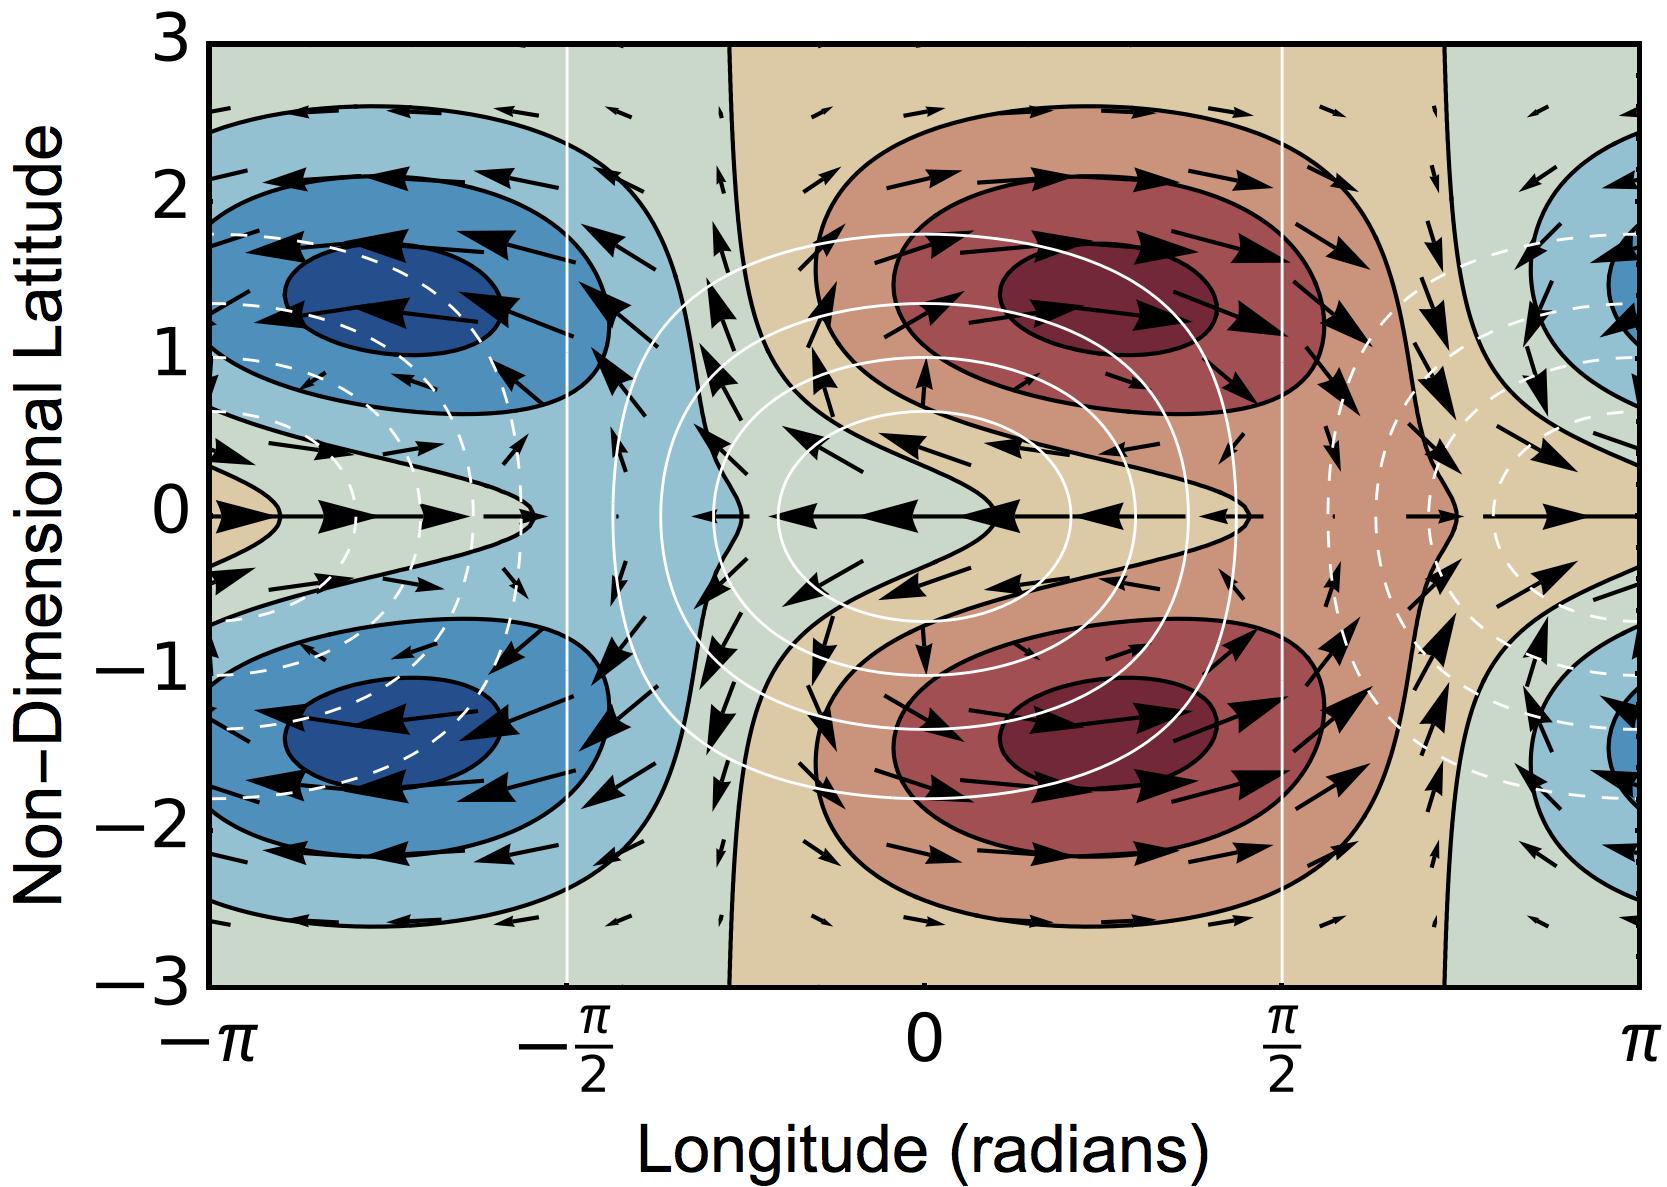
\includegraphics[width=1.0\textwidth]{figures/wave-mean-flow/motivate-tsai.png}
    \caption{motivate-tsai.}
    \label{fig:motivate-tsai}
  \end{subfigure}
  \caption{Forced solutions.}
  \label{fig:motivate-showman-tsai}
\end{figure}


%SECTION CONCLUSIONS

In this section, I introduced the free and forced solutions of a linear shallow-water system on a beta-plane.


%%%%%%%%%%%%%%%%%%%%%%%%%%%%%%%%%%%%

%SECTION 2 --
\section{Zonal Acceleration of Equatorial Jet}\label{sec:zonal-acceleration}

This shallow-water system shows which stationary waves will be excited in the atmosphere of a tidally locked planet by the day-night forcing. The next step is to calculate the zonal acceleration produced by these stationary waves, and find the effect of the resulting flow on the waves themselves.

I will follow \citet{showman2010superrotation} and \citet{showman2011superrotation} to show that the classic Matsuno-Gill model introduced in the previous section predicts zero acceleration at the equator. An addition momentum transport term is required to represent the asymmetric momentum forcing due to vertical transport on the day- and night-sides \citet{shell2004superrotation}.


%SUBSECTION --
\subsection{Acceleration in a Matsuno-Gill Model}

Zonally averaging the zonal momentum equation in Equation \ref{eqn:sw-eqns-1} \citep{thuburn1999zonalmean} \citep{showman2010superrotation} gives the zonal acceleration profile in the shallow-water model:

\begin{equation}\label{eqn:zonal-mean-mom}
  \frac { \partial \overline { u } } { \partial t } = \underbrace { \overline { v } ^ { * } \left[ f - \frac { \partial \overline { u } } { \partial y } \right] } _ { I } \underbrace { - \frac { 1 } { \overline { h } } \frac { \partial } { \partial y } \left[ \overline { ( h v ) ^ { \prime } u ^ { \prime } } \right] } _ { I I } + \underbrace {  \frac { 1 } { \overline { h } } \overline { u ^ { \prime } Q ^ { \prime } } } _ { I I I } \underbrace { - \frac { \overline { u } ^ { * } } { \tau _ { \mathrm { drag } } } } _ { I V } - \frac { 1 } { \overline { h } } \frac { \partial \left( \overline { h ^ { \prime } u ^ { \prime } } \right) } { \partial t }
\end{equation}

Figure \ref{fig:matsuno-zonal-acceleration-terms} shows the different components of Equation \ref{eqn:zonal-mean-mom} for the classic system of \citet{matsuno1966quasi}:

\begin{itemize}
  \item Green line: Term I, zonal momentum transport by mean meridional circulation
  \item Red line: Term II, horizontal transport of zonal momentum
  \item Blue line: Term III, vertical transport of zonal eddy momentum
  \item Purple line: Term IV, zonal drag
  \item Black line: Left-hand-side, sum of all four terms.
\end{itemize}

Note that there is no contribution from the final term in Equation \ref{eqn:zonal-mean-mom} as the solution is stationary.

The key point from Figure \ref{fig:matsuno-zonal-acceleration-terms} is that there is zero zonal acceleration at the equator, so this model is not consistent with GCM simulations of tidally locked planets that show equatorial superrotation at the equator.

\begin{figure}
  \centering
  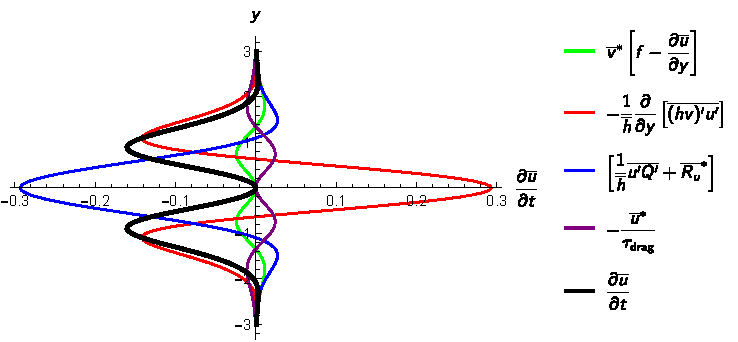
\includegraphics[width=0.85\textwidth]{figures/wave-mean-flow/matsuno-zonal-acceleration-terms.pdf}
  \caption{Acceleration terms.}
  \label{fig:matsuno-zonal-acceleration-terms}
\end{figure}


We can show that the acceleration must be zero at the equator for these forced shallow-water equations. Rewriting the zonal mean momentum equation in terms of the relative vorticity $\zeta$ \citep{thuburn1999zonalmean} \citep{showman2011superrotation}

\begin{equation}
  \frac { \partial \overline { u } } { \partial t } = \overline { v ^ { \prime } \zeta ^ { \prime } } + \overline { v } ( f + \overline { \zeta } ) - \frac { \overline { u } } { \tau _ { \mathrm { drag } } } + \overline { R _ { u } },
\end{equation}

we see that as $v=0$ at the equator (due to the symmetric forcing in $y$) $\frac { \partial \overline { u } } { \partial t } = 0$ at the equator also.

The fact that there is in the GCM simulations shows another process is affecting the zonal momentum at the equator. Note that this condition still applies to the same equations linearised about a zonal flow $\bar{U}(y)$ (Equation X).


% This also is necessary from the zonal momentum equation (the first line of Equation \ref{eqn:sw-eqns-1}). As the day-night forcing is symmetric about the equatorial, the meridional velocity $v$ must be zero at the equator. Also, the forcing $Q$ varies sinusoidally with $x$, so produces a sinusoidal response in $h$ along the equator, which will have a zonal mean of zero. Therefore, the zonal momentum equation requires that there is no zonal mean acceleration at the equator.


%SUBSECTION --
\subsection{Correction to Vertical Momentum Transport}

The forced shallow-water equations predict zero zonal acceleration at the equator. So, there must be another process at work at the equator producing the eastward zonal flow seen in GCM simulations.

\citet{showman2011superrotation} invoke a correction to the zonal momentum equation from \citet{shell2004superrotation}.

\begin{equation}\label{eqn:sw-eqns-R}
  \begin{gathered}
     \frac{\partial u}{\partial t} - \beta y v +\frac{\partial h}{\partial x} = R_{u} \\
      \frac{\partial v}{\partial t} + \beta y u + \frac{\partial h}{\partial y} = 0 \\
    \frac{\partial h}{\partial t} +c^{2}(\frac{\partial u}{\partial x} + \frac{\partial v}{\partial y}) = Q(x,y) \\
  \end{gathered}
\end{equation}

The correction $R_{u}$ represents the effect of exchanging zonal momentum between the active layer and the lower layer. On the day-side, air with zero angular momentum rises from the substellar point into the active layer, giving a zonal acceleration which opposes the local $u$ field. To conserve the vertically integrated local zonal momentum this acceleration is $R_{u} - \frac { Q u } { h }$ \citep{showman2011superrotation}. On the night-side, air leaves the active layer which does not affect the local angular momentum, so $R_{u}=0$.

\begin{equation}
   R _{u}  = \left \begin{array} { l l } { - \frac { Q u } { h } , } & { Q > 0 } \\ { 0 , } & { Q < 0 } \end{array} \right
\end{equation}

This modifies the zonal mean momentum equation to:

\begin{equation}\label{eqn:zonal-mean-mom-with-R}
  \frac { \partial \overline { u } } { \partial t } = \underbrace { \overline { v } ^ { * } \left[ f - \frac { \partial \overline { u } } { \partial y } \right] } _ { I } \underbrace { - \frac { 1 } { \overline { h } } \frac { \partial } { \partial y } \left[ \overline { ( h v ) ^ { \prime } u ^ { \prime } } \right] } _ { I I } + \underbrace { \left[ \frac { 1 } { \overline { h } } \overline { u ^ { \prime } Q ^ { \prime } } + \overline { R _ { u } } ^ { * } \right] } _ { I I I } \underbrace { - \frac { \overline { u } ^ { * } } { \tau _ { \mathrm { drag } } } } _ { I V } - \frac { 1 } { \overline { h } } \frac { \partial \left( \overline { h ^ { \prime } u ^ { \prime } } \right) } { \partial t }
\end{equation}

Figure \ref{fig:matsuno-zonal-acceleration-terms-with-R} shows the terms Equation \ref{eqn:zonal-mean-mom-with-R}. In comparison to Figure \ref{fig:matsuno-zonal-acceleration-terms}, there is now a zonal acceleration at the equator.

\begin{figure}
  \centering
  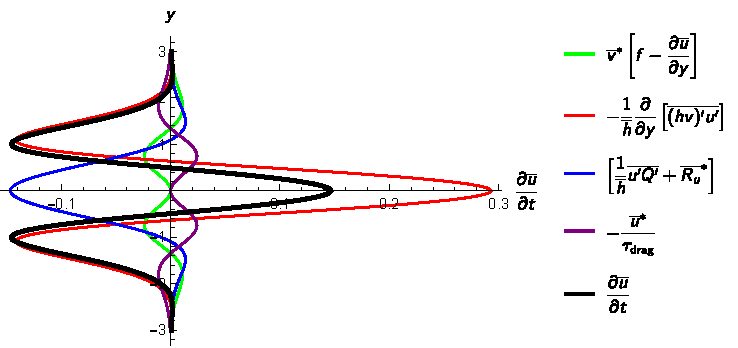
\includegraphics[width=0.85\textwidth]{figures/wave-mean-flow/matsuno-zonal-acceleration-terms-with-R.pdf}
  \caption{Acceleration terms with R.}
  \label{fig:matsuno-zonal-acceleration-terms-with-R}
\end{figure}

Rewriting the zonal mean momentum equation in terms of the relative vorticity again shows that there is now a non-zero acceleration at the equator due to $R_{u}$:

\begin{equation}
  \frac { \partial \overline { u } } { \partial t } = \overline { v ^ { \prime } \zeta ^ { \prime } } + \overline { v } ( f + \overline { \zeta } ) - \frac { \overline { u } } { \tau _ { \mathrm { drag } } } + \overline { R _ { u } },
\end{equation}

This explains the equatorial superrotation on tidally locked planets. But, it does not explain why momentum-conserving retrograde westward flow predicted by this shallow-water model in the mid-latitudes, does not appear in the GCM simulations, which instead have an atmosphere superrotating at most latitudes. In Chapter XX I will discuss this.


%SUBSECTION --
\subsection{Horizontal Momentum Transport from Stationary Waves}

It is helpful to now consider the terms in Equation \ref{eqn:zonal-mean-mom} in more detail.

Term II in Equation \ref{eqn:zonal-mean-mom} is the horizontal momentum transport. The sign of Term II depends on the

But, it is cancelled out by the vertical momentum transport.

%SUBSECTION --
\subsection{Equilibrium Equatorial Flow}

This provides an estimate of the equilibrium zonal flow speed on the equator, which will occur when $\frac { \partial \overline { u } } { \partial t }=0$:

\begin{equation}
  \frac { \overline { u } } { \tau _ { \mathrm { drag } } } = \overline { R _ { u } },
\end{equation}

As the zonal flow $\overline { u }$ increases, the drag term $\frac { \overline { u } } { \tau _ { \mathrm { drag } } }$ will increase until it balances the acceleration due to vertical momentum transport $\overline { R _ { u } }$.

The acceleration due to vertical momentum transport $\overline { R _ { u } }$ will also decrease as the zonal flow $\overline { u }$ increases, so even if $\tau_{drag}$ is very large and  $\frac { \overline { u } } { \tau _ { \mathrm { drag } } }$ is negligible, $\overline { R _ { u } }$ will eventually become zero for large enough zonal flow, and the acceleration will become zero. \citet{showman2011superrotation} suggest that $\overline { R _ { u } }$ simply gets smaller as the zonal mean $\overline{u}$ gets larger. Later, I will add the fact that the forced response is Doppler-shifted eastwards, changing the part of the eddy response that is on the day-side and contributes to $\overline { R _ { u } }$.

In addition, I will show how this eastward shift decreases term II in Equation \ref{eqn:zonal-mean-mom-with-R} by shifting the different wave components closer together. This further decreases the equatorial acceleration as the zonal flow increases, making it reach an equilibrium sooner.

%SECTION CONCLUSIONS



%%%%%%%%%%%%%%%%%%%%%%%%%%%%%%%%%%%%
%SECTION X -- NONLINEAR SHALLOW
\section{Zonal Acceleration of Midlatitude Jets in Linear Model}

%SUBSECTION --
\subsection{Problem with Equatorial Jet Only}



GCM results show an atmosphere, and a jet layer, with positive net angular momentum. Often the jet layer is superrotating at all latitudes.

The Showman linear shallow-water model can only have negative angular momentum in the jet layer, and always predicts midlatitude easterly flow. Figure X shows the acceleration profile from Showman. Note that this must have easterly flow above a certain latitude, and must have negative total angular momentum.

Compare to Figure X, which shows the velocity profile from the GCM with flow at all latitudes. Refs X, X, and X all show prograde flow at all latitudes.

So, the linear model contradicts:

\begin{enumerate}
  \item Positive net angular momentum in the jet layer in the GCM
  \item Cases with prograde flow at all latitudes in the GCM
  \item Positive total angular momentum in the whole atmosphere in the GCM
\end{enumerate}

So, there is something missing from the shallow-water model.

\begin{figure*}
  \centering
  \gridline{\fig{figures/eqm-zonal-flow/sp-accn.png}{0.32\textwidth}{Shallow-water acceleration}
            \fig{figures/eqm-zonal-flow/tide-zonal-flow-profile.pdf}{0.32\textwidth}{Mean zonal flow at -15.}
            \fig{figures/eqm-zonal-flow/jet-layer-m.pdf}{0.32\textwidth}{AM evolution}}
  \caption{Predicted acceleration and GCM features it is not consistent with.}
  \label{fig:day-1-tide-aci}
\end{figure*}


\subsection{Gierasch Mechanism on a Tidally Locked Planet}


The nature of the meridional circulation in the atmosphere of a tidally locked planet has not been addressed in detail. REFS have discussed the formation of subtropical jets or different meridional circulations on the day- and night-sides, but there is no consistent theory of its behaviour and effects.

The longitudinally varying forcing makes it more complex than the axisymmetric meridional circulation on a non-tidally locked planet. In addition, the strong day-night zonal circulation would appear to be much more important. We suggest that the meridional circulation is in fact also a vital part of the global circulation, particularly in the formation of the superrotating zonal flow.

We suggest that the meridional circulation on a tidally locked planet can be considered as a zonal-mean quantity despite the strong longitudinal variation in forcing.

This is due to the linearity of the meridonal circulation -- in all of its zonal and meridional velocities, and meridional momentum flux -- with respect to forcing. Before any perturbations form, we can consider each longitude separately. HH show that each of these quantities are linear with response to the forcing, and this is true at each longitude. In the axisymmetric case with meridionally varying forcing $Q(\phi) = Q_{0}\cos{\phi}$, the zonal mean of any quantity is:

\begin{equation}
  \overline{X} \sim \overline{Q} = Q(\phi)=Q_{0}\cos{\phi}.
\end{equation}

For the same forcing on a tidally locked planet, the forcing is $ Q(\phi,\lambda)=Q_{0}\cos{\phi}\sin{\lamda}$ on the day-side, and a uniform relaxation on the night-side (which has no effect here). So, the zonal mean is:

\begin{equation}
  \overline{X} \sim \overline{Q} = Q(\phi,\lambda)=Q_{0}\cos{\phi}\overline{\sin\lambda},
\end{equation}

where the mean of the $\sin \lambda$ is only taken over the day-side, giving:

\begin{equation}
  \overline{X} \sim Q_{0}\cos{\phi}\frac{2}{2} = Q_{0}\cos{\phi},
\end{equation}

where the $2$ in the denominator comes from the fact that the forcing is only applied to half the longitudes.

So, when non-linear effects and zonal flow are not important, all parts of the meridional circulation are linear with the forcing strength, and the longitudinal distribution of the forcing does not matter. So, we can consider the effect of the meridional circulation on the zonal-mean winds and momentum fluxes by just considering its zonal mean quantities (which are identical to the axisymmetric case), even though their longitudinal distribution may be very different to the axisymmetric case.

Figure X shows this non-dependence on the longitudinal form of the forcing. On the first day of spin-up, the mass streamfunctions are the same for each forcing case, showing the same overturning. Also, the zonal winds due to either axisymmetric or tidally locked forcing are the same. But, Figure X shows that their distribution in longitude is very different. Then, Figure X shows that once the perturbations are larger and the zonal flow forms they are very different.

But, this shows that we can simplify our thinking about the meridional circulation by considering the zonal mean. In the next section, we will use this to suggest the role of the meridional circulation in the formation of the zonal mean. We will use a mechanism previously applied to non-tidally locked planets.


\subsection{Demonstration of Mechanism in GCM}

In this section, I will focus on two simulations to demonstrate the proposed mechanism. Later I will present a suite of simulations.

Figure X shows day 1 zonal wind, surface wind, and streamfunction for tide and axi. Show mean streamfunction of tide and axi -- there is a non-zero streamfunction in the tide case, which would not be true if it were totally sinusoidally forced as in SP2011.


\begin{figure}
  \centering
  \begin{subfigure}[t]{0.32\textwidth}
    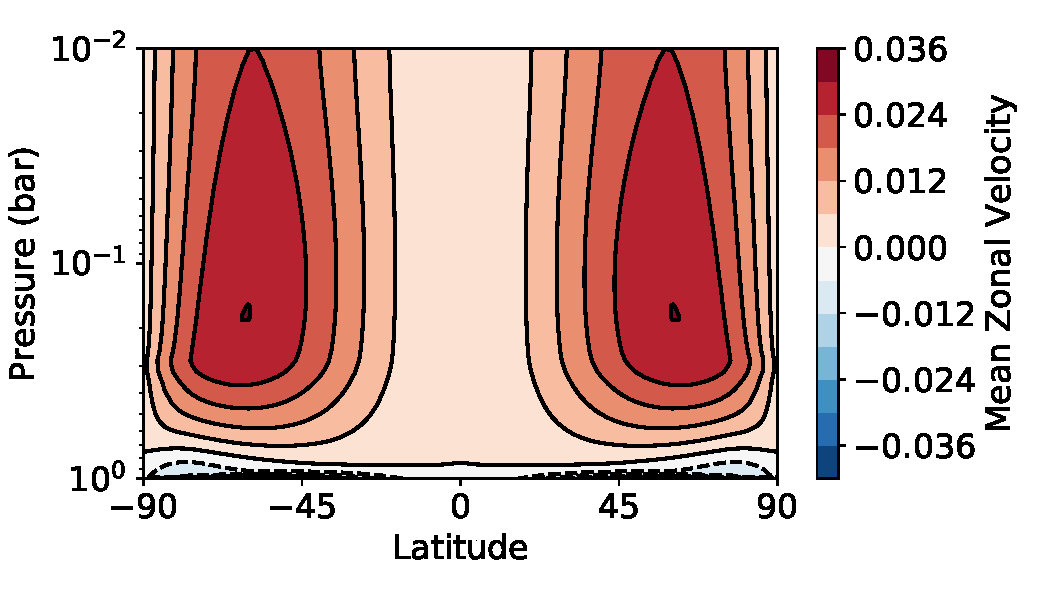
\includegraphics[width=\textwidth]{figures/eqm-zonal-flow/tide_1_u.pdf}
    \caption{Zonal-mean zonal velocity.}
  \end{subfigure}
  %
  \begin{subfigure}[t]{0.32\textwidth}
    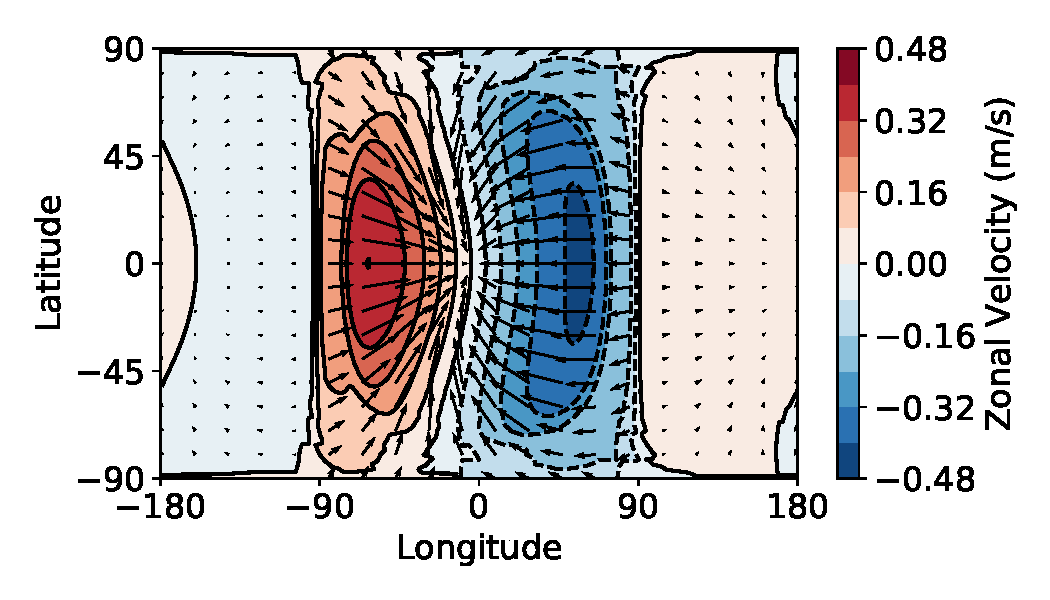
\includegraphics[width=\textwidth]{figures/eqm-zonal-flow/tide_1_surf_ucomp.pdf}
    \caption{Zonal velocity.}
  \end{subfigure}
  %
  \begin{subfigure}[t]{0.32\textwidth}
    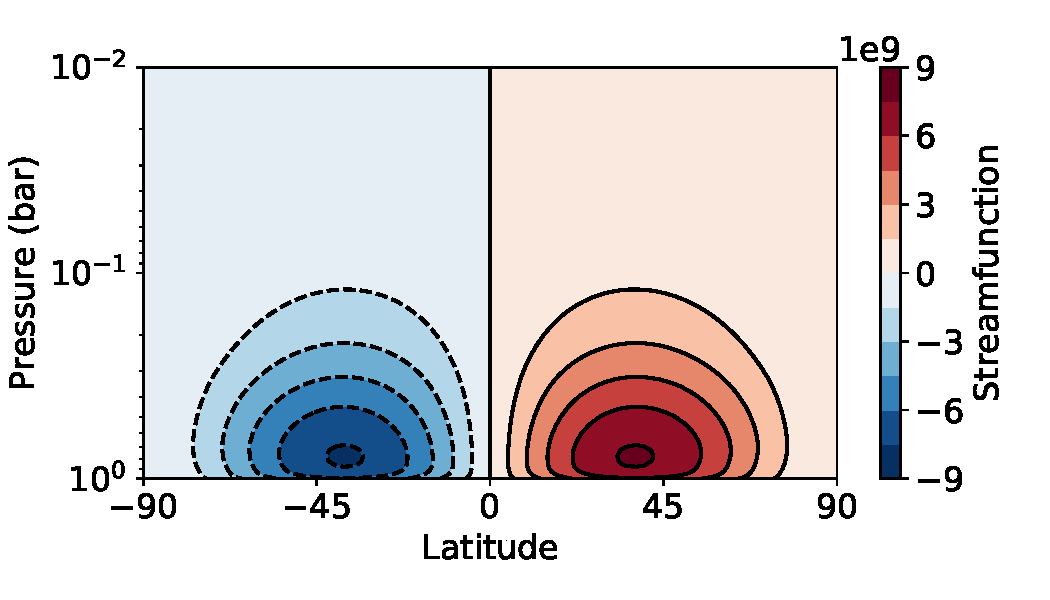
\includegraphics[width=\textwidth]{figures/eqm-zonal-flow/sf_tide_day1.pdf}
    \caption{Streamfunction}
  \end{subfigure}
  \\
  \begin{subfigure}[t]{0.32\textwidth}
    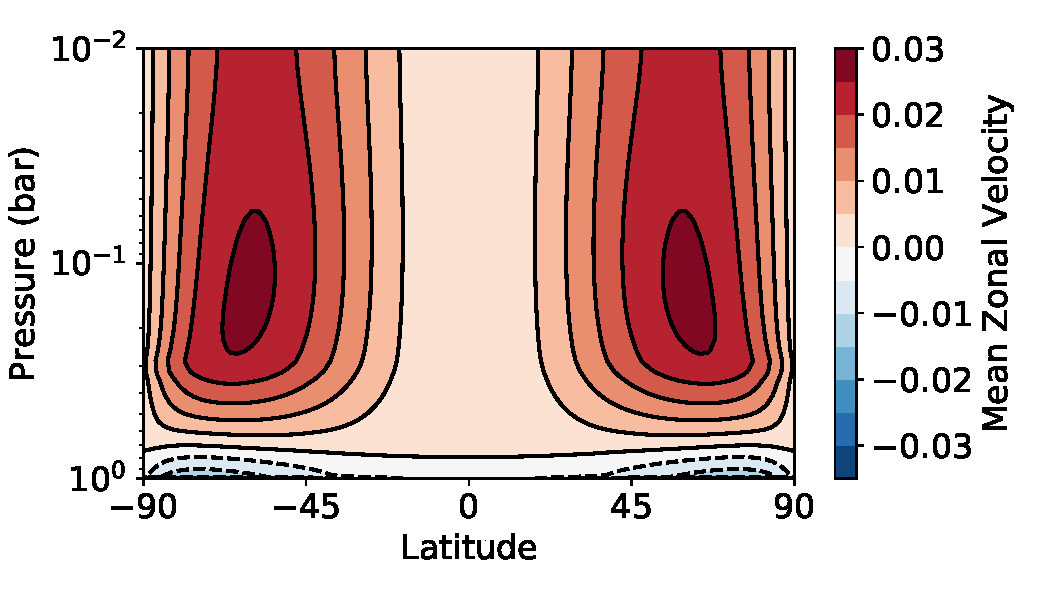
\includegraphics[width=\textwidth]{figures/eqm-zonal-flow/axi_1_u.pdf}
    \caption{Zonal-mean zonal velocity.}
  \end{subfigure}
  %
  \begin{subfigure}[t]{0.32\textwidth}
    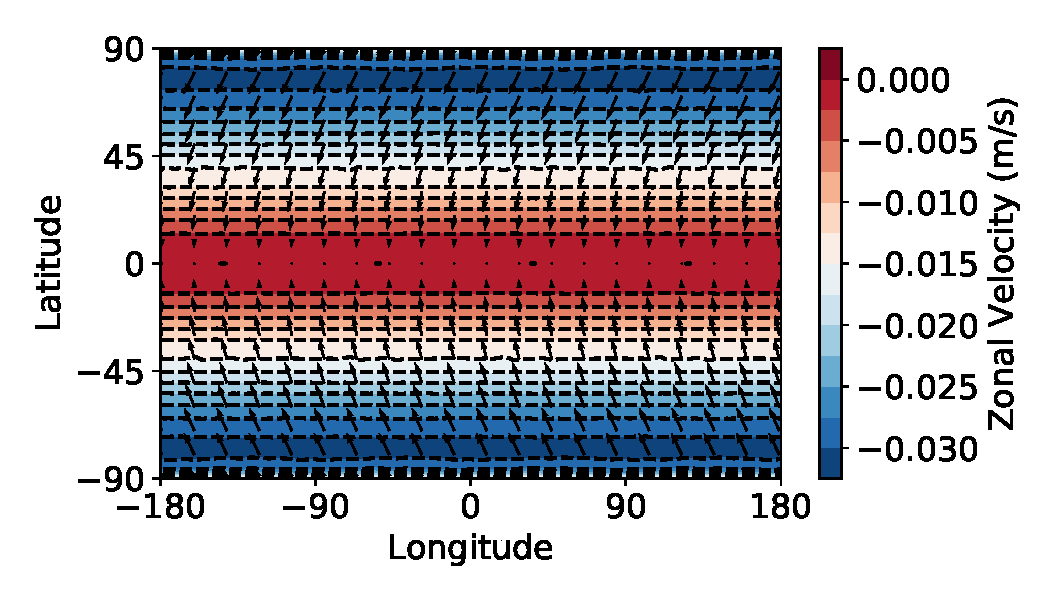
\includegraphics[width=\textwidth]{figures/eqm-zonal-flow/axi_1_surf_ucomp.pdf}
    \caption{Zonal velocity.}
  \end{subfigure}
  %
  \begin{subfigure}[t]{0.32\textwidth}
    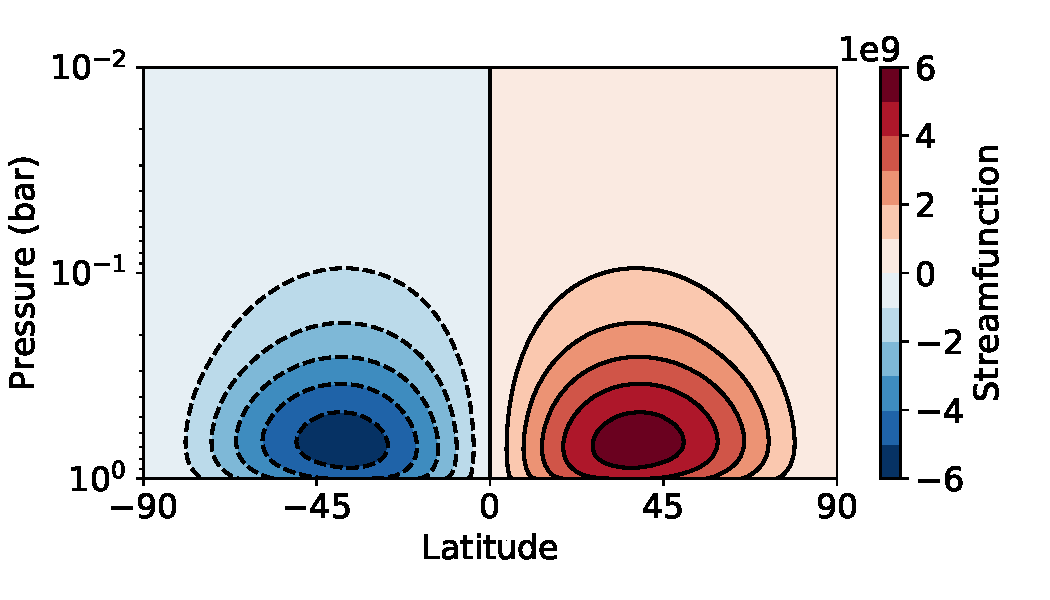
\includegraphics[width=\textwidth]{figures/eqm-zonal-flow/sf_axi_day1.pdf}
    \caption{Streamfunction}
  \end{subfigure}
  \caption{Day 1 of tide and axi.}
  \label{fig:day-1-tide-aci}
\end{figure}

Show evolution of zonal wind field. Tide and axi are the same on the first day, due to linearity argument above. Show surface wind maps of tide and axi on first day, they are very different but have the same zonal mean. Axi evolves as expected. Horizontal transport kicks in on tide, producing equatorial superrotation.



\begin{figure}
  \centering
  \begin{subfigure}[t]{0.32\textwidth}
    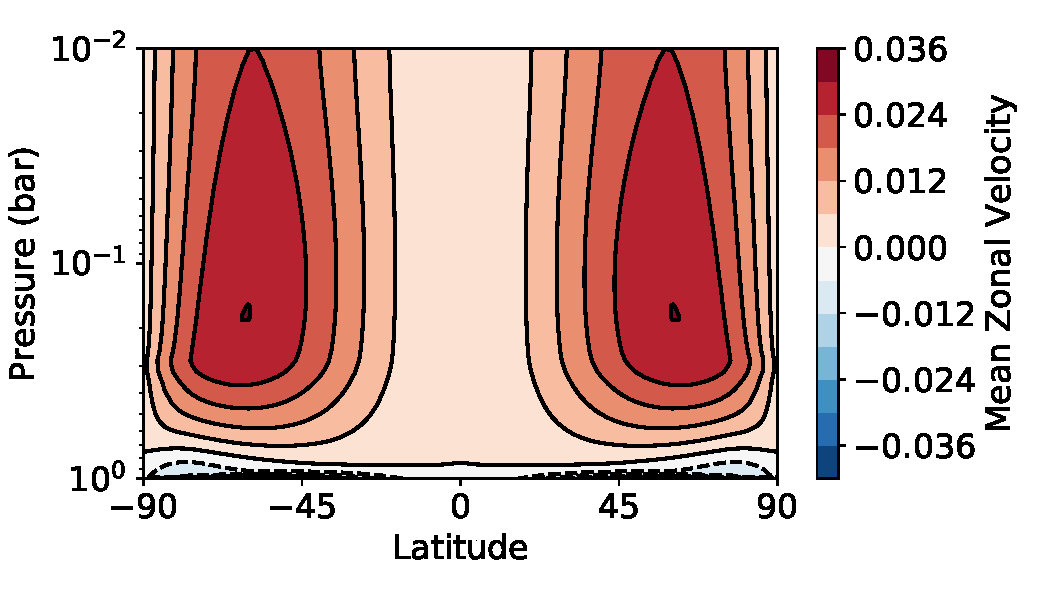
\includegraphics[width=\textwidth]{figures/eqm-zonal-flow/tide_1_u.pdf}
    \caption{1 day}
  \end{subfigure}
  %
  \begin{subfigure}[t]{0.32\textwidth}
    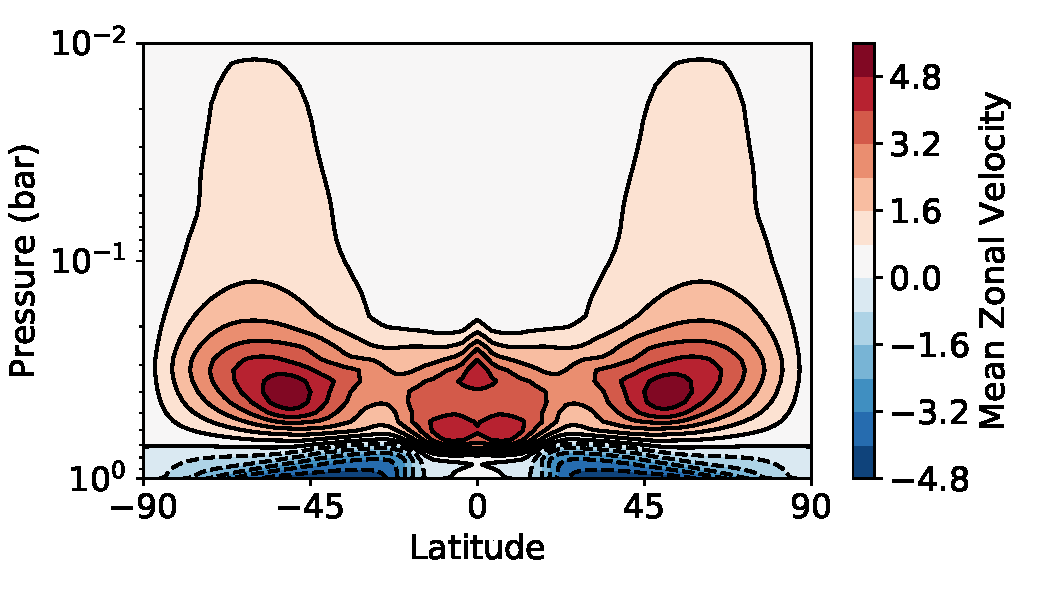
\includegraphics[width=\textwidth]{figures/eqm-zonal-flow/tide_10_u.pdf}
    \caption{10 days}
  \end{subfigure}
  %
  \begin{subfigure}[t]{0.32\textwidth}
    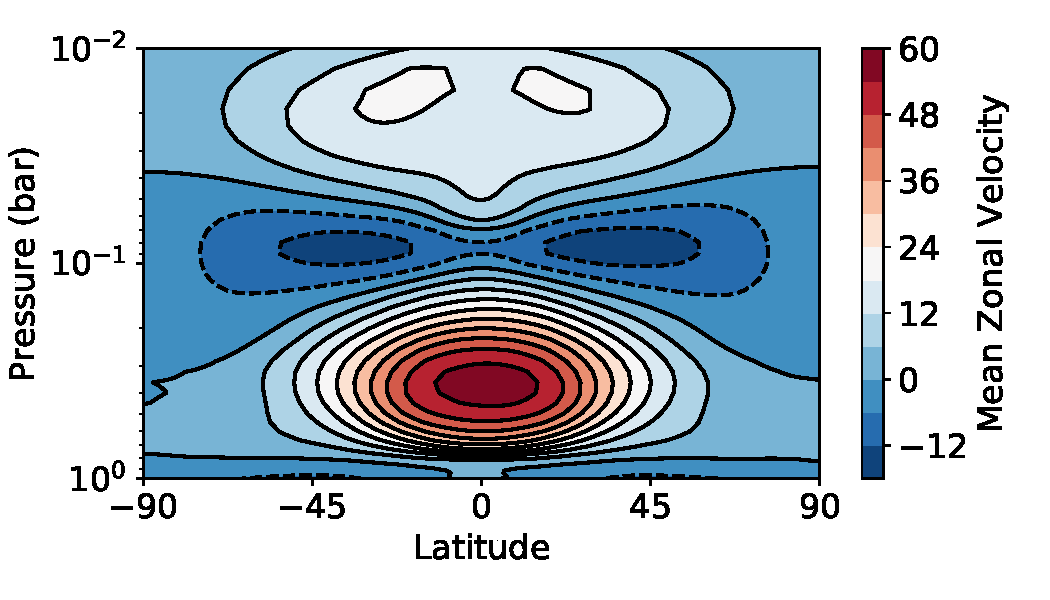
\includegraphics[width=\textwidth]{figures/eqm-zonal-flow/tide_500_u.pdf}
    \caption{500 days}
  \end{subfigure}
  \\
  \begin{subfigure}[t]{0.32\textwidth}
    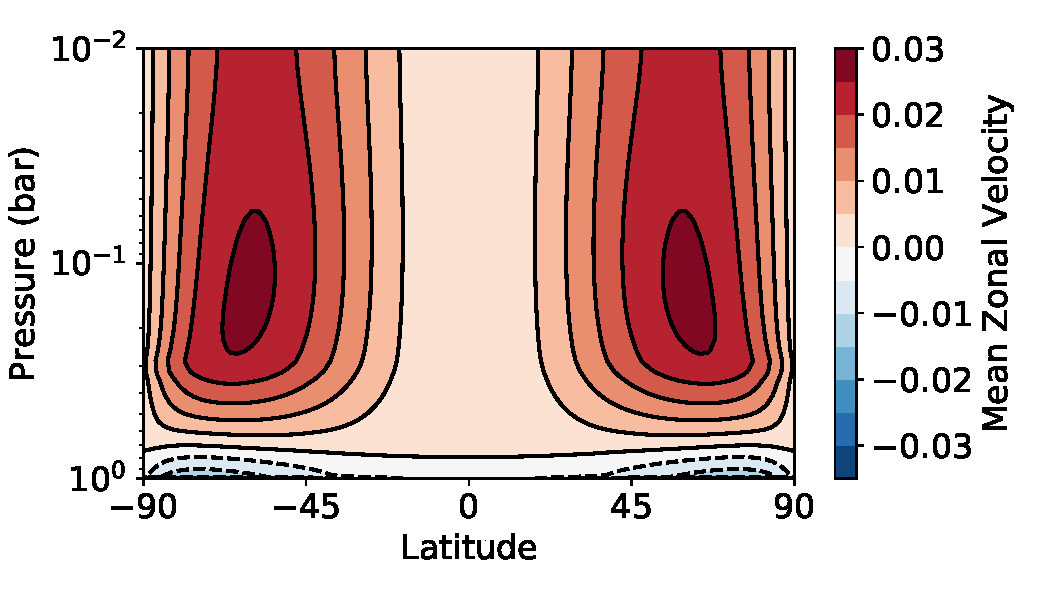
\includegraphics[width=\textwidth]{figures/eqm-zonal-flow/axi_1_u.pdf}
    \caption{1 day}
  \end{subfigure}
  %
  \begin{subfigure}[t]{0.32\textwidth}
    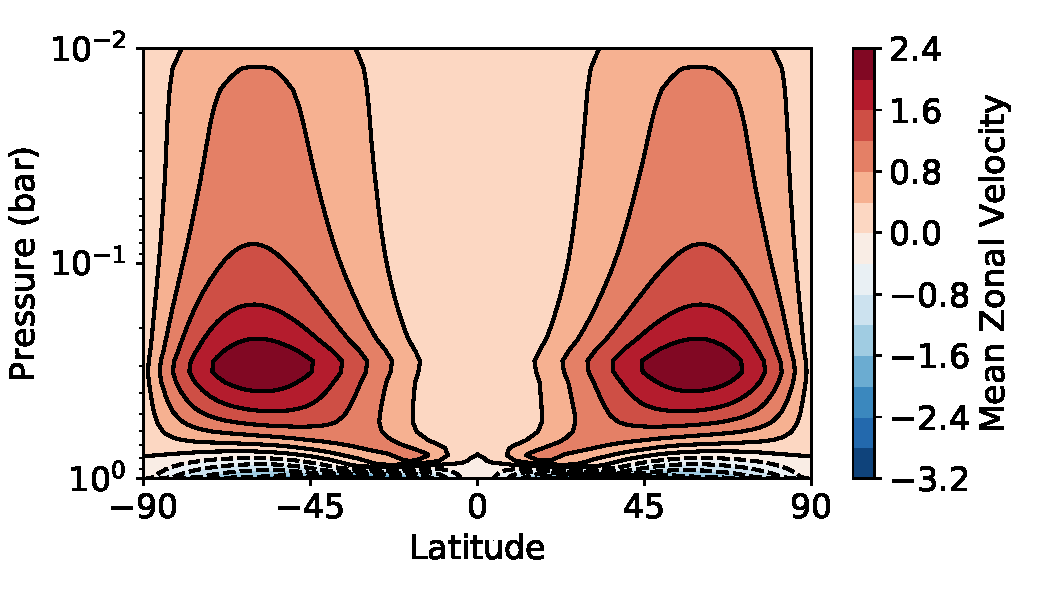
\includegraphics[width=\textwidth]{figures/eqm-zonal-flow/axi_10_u.pdf}
    \caption{10 days}
  \end{subfigure}
  %
  \begin{subfigure}[t]{0.32\textwidth}
    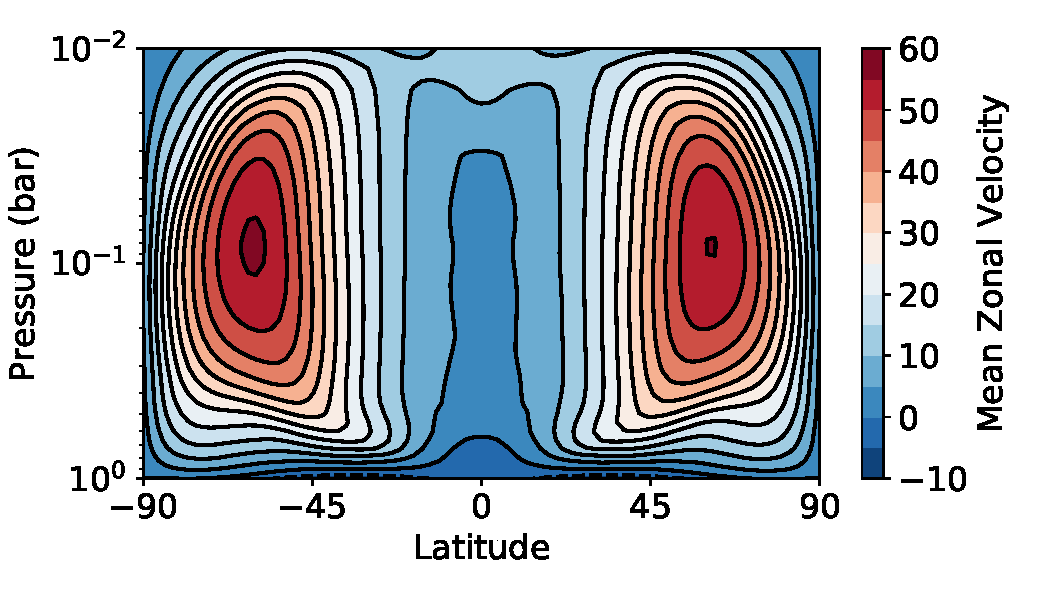
\includegraphics[width=\textwidth]{figures/eqm-zonal-flow/axi_500_u.pdf}
    \caption{500 days}
  \end{subfigure}
  \caption{Zonal velocity and drag}
  \label{fig:default-gcm-velocity-drag}
\end{figure}


\subsection{Fluxes of Mechanism in GCM}

Show all fluxes for tide and axi. Same mean meridional term?

\begin{figure}
  \centering
  \begin{subfigure}[t]{0.45\textwidth}
    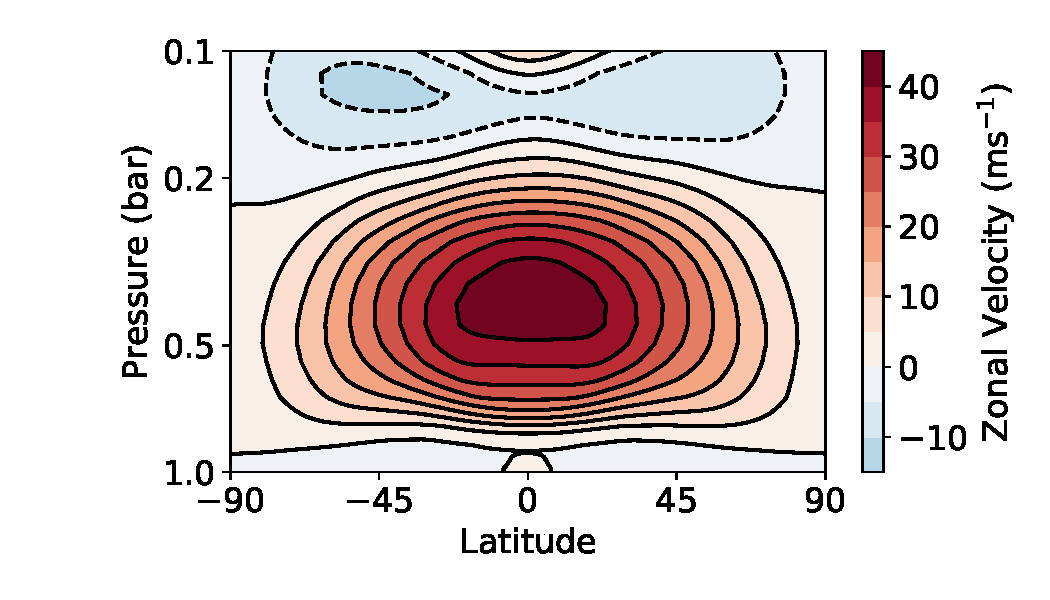
\includegraphics[width=\textwidth]{figures/eqm-zonal-flow/5_flux.pdf}
    \caption{Zonal-mean zonal velocity.}
  \end{subfigure}
  %
  \begin{subfigure}[t]{0.45\textwidth}
    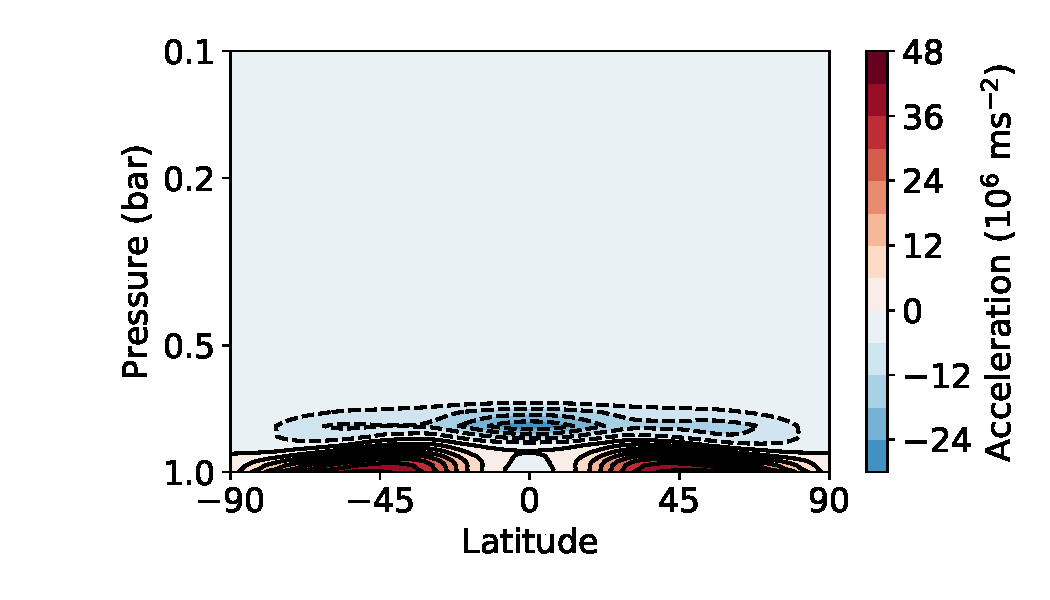
\includegraphics[width=\textwidth]{figures/eqm-zonal-flow/4_flux.pdf}
    \caption{Acceleration due to Rayleigh drag.}
  \end{subfigure}
  \caption{Zonal velocity and drag}
  \label{fig:default-gcm-velocity-drag}
\end{figure}

\begin{figure}
  \centering
  \begin{subfigure}[t]{0.45\textwidth}
    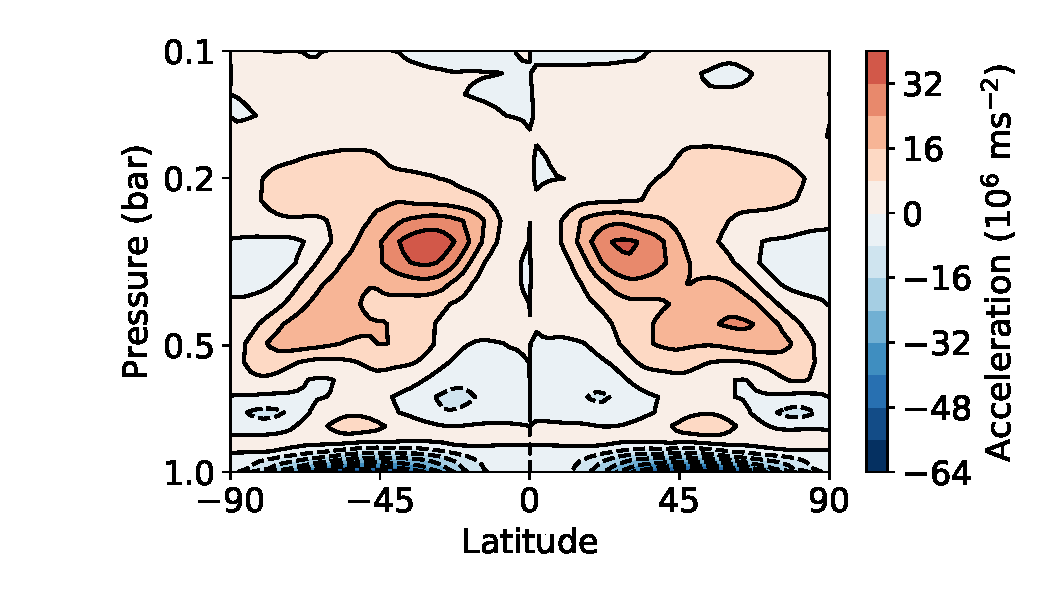
\includegraphics[width=\textwidth]{figures/eqm-zonal-flow/0_flux.pdf}
    \caption{Mean horizontal.}
  \end{subfigure}
  %
  \begin{subfigure}[t]{0.45\textwidth}
    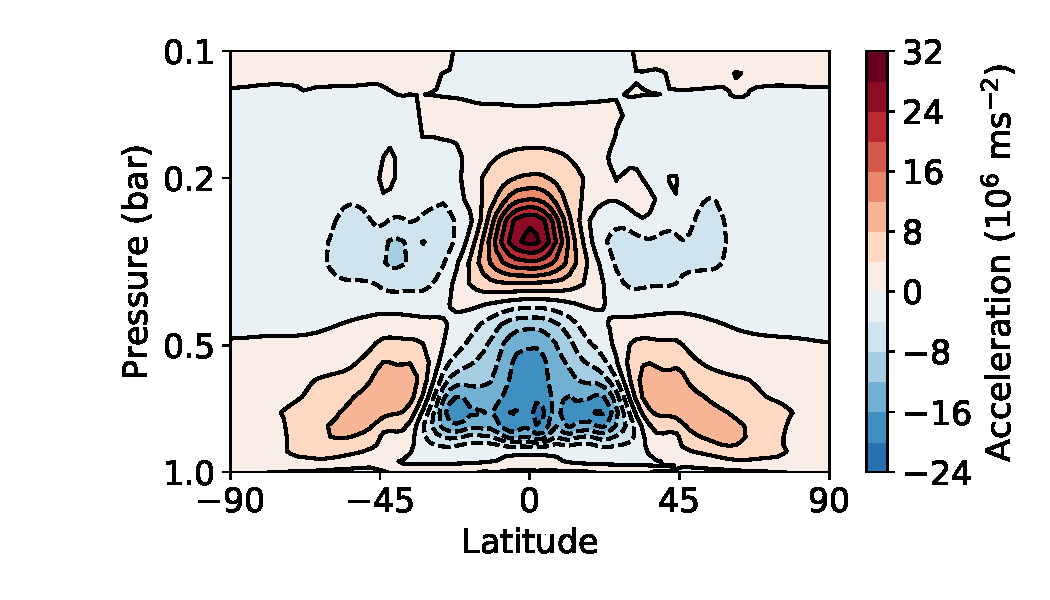
\includegraphics[width=\textwidth]{figures/eqm-zonal-flow/1_flux.pdf}
    \caption{Mean vertical.}
  \end{subfigure}
  \\
  \begin{subfigure}[t]{0.45\textwidth}
    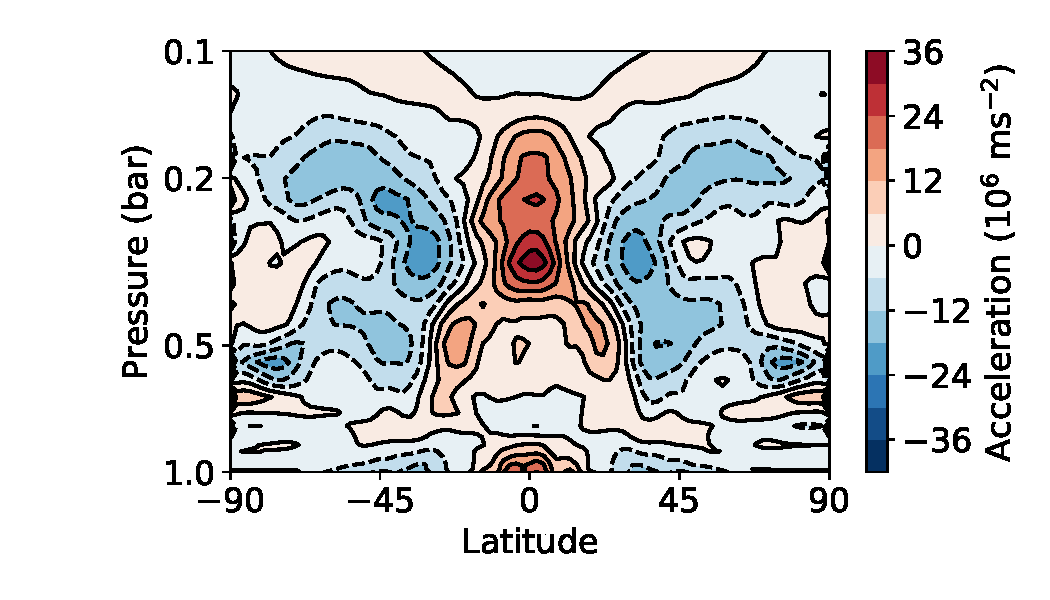
\includegraphics[width=\textwidth]{figures/eqm-zonal-flow/2_flux.pdf}
    \caption{Stationary horizontal.}
  \end{subfigure}
  %
  \begin{subfigure}[t]{0.45\textwidth}
    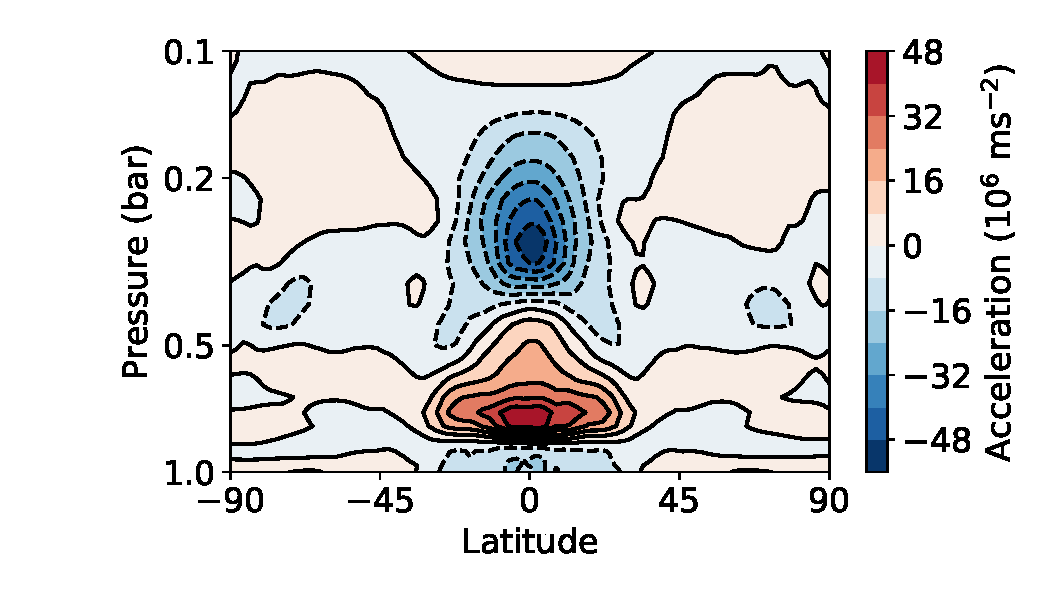
\includegraphics[width=\textwidth]{figures/eqm-zonal-flow/3_flux.pdf}
    \caption{Stationary vertical.}
  \end{subfigure}
  \caption{Mean and eddy acceleration.}
  \label{fig:default-gcm-accelerations}
\end{figure}




%SECTION CONCLUSIONS



%%%%%%%%%%%%%%%%%%%%%%%%%%%%%%%%%%%%
\section{Linear Model}

Linearise about subtropical jets like ZG and Held. Show that acceleration is similar. Vary subtropical jet strength.

Vary Gaussian jet to get zero acceleration. Show that without subtropical jets, always get retro flow at high lats. Show that with subtropical jets, can have balanced prograde flow everywhere.

%%%%%%%%%%%%%%%%%%%%%%%%%%%%%%%%%%%%
%SECTION X -- NONLINEAR SHALLOW
\section{Nonlinear Shallow-Water Model}

We can demonstrate this most easily in a non-linear shallow-water model.

The real forcing is approximately the sum of a sinusoid forcing the SP circulation, and a mean forcing producing the meridional circulation and subtropical jets.

We can expand the real forcing as a sum of terms to see that these are the two largest terms.

Test 1: sin Forcing

Test 2: sin with flat night-side and global prograde

Test 3: sin with flat night-side and high lat retrograde

Momentum balance


%SUBSECTION --
\subsection{Momentum Balance}

%SECTION CONCLUSIONS



%%%%%%%%%%%%%%%%%%%%%%%%%%%%%%%%%%%%
%SECTION X -- GCM
\section{Zonal Flow Scaling Regimes}

%SUBSECTION --
\subsection{Scaling}

Relative strength of equatorial and subtropical jets in SW model, and GCM

%SUBSECTION --
\subsection{Non-Linear Model Tests}

\begin{figure}
  \centering
  \begin{subfigure}[t]{0.45\textwidth}
    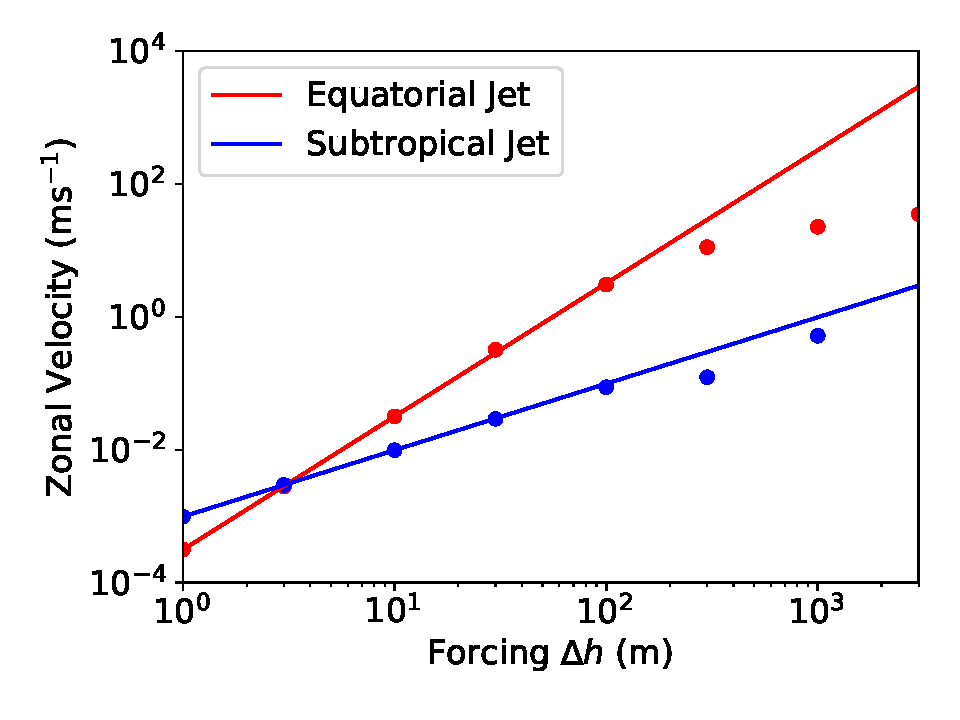
\includegraphics[width=\textwidth]{figures/eqm-zonal-flow/u_Q_scaling.pdf}
    \caption{Scaling with Q.}
  \end{subfigure}
  %
  \begin{subfigure}[t]{0.45\textwidth}
    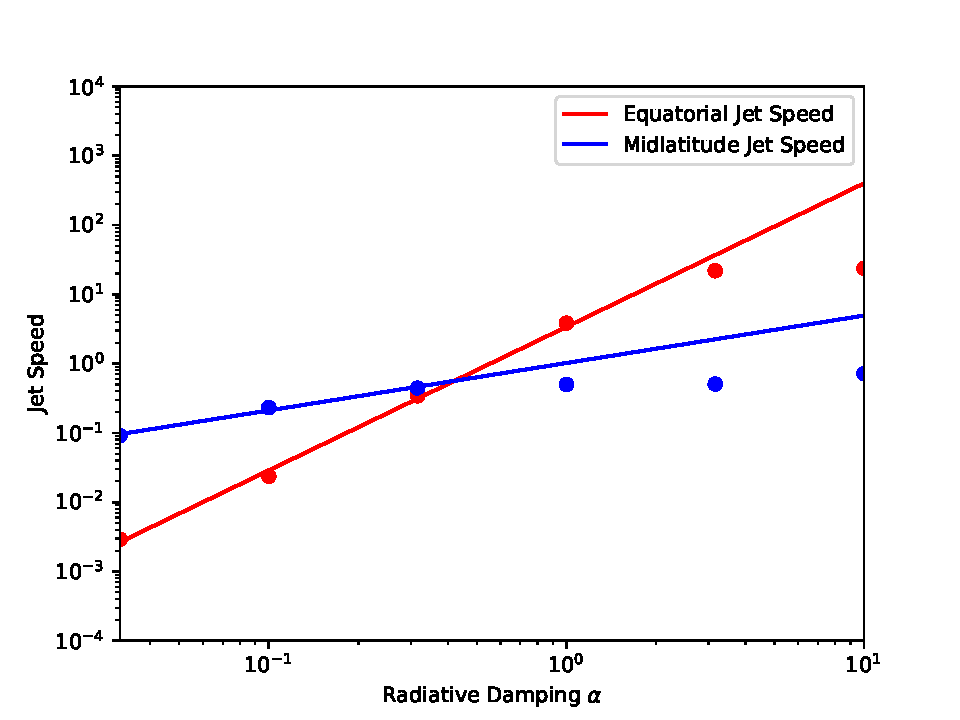
\includegraphics[width=\textwidth]{figures/eqm-zonal-flow/u_alpha_scaling.pdf}
    \caption{Scaling with damping.}
  \end{subfigure}
  \caption{Jet scaling in non-linear model.}
  \label{fig:nonlin-u-scaling}
\end{figure}


%SUBSECTION --
\subsection{GCM Tests}

Suite of tests like in review, explain one, two, three jets, retrograde jets.

Test predicted scaling

\begin{figure}
  \centering
  \begin{subfigure}[b]{0.32\textwidth}
    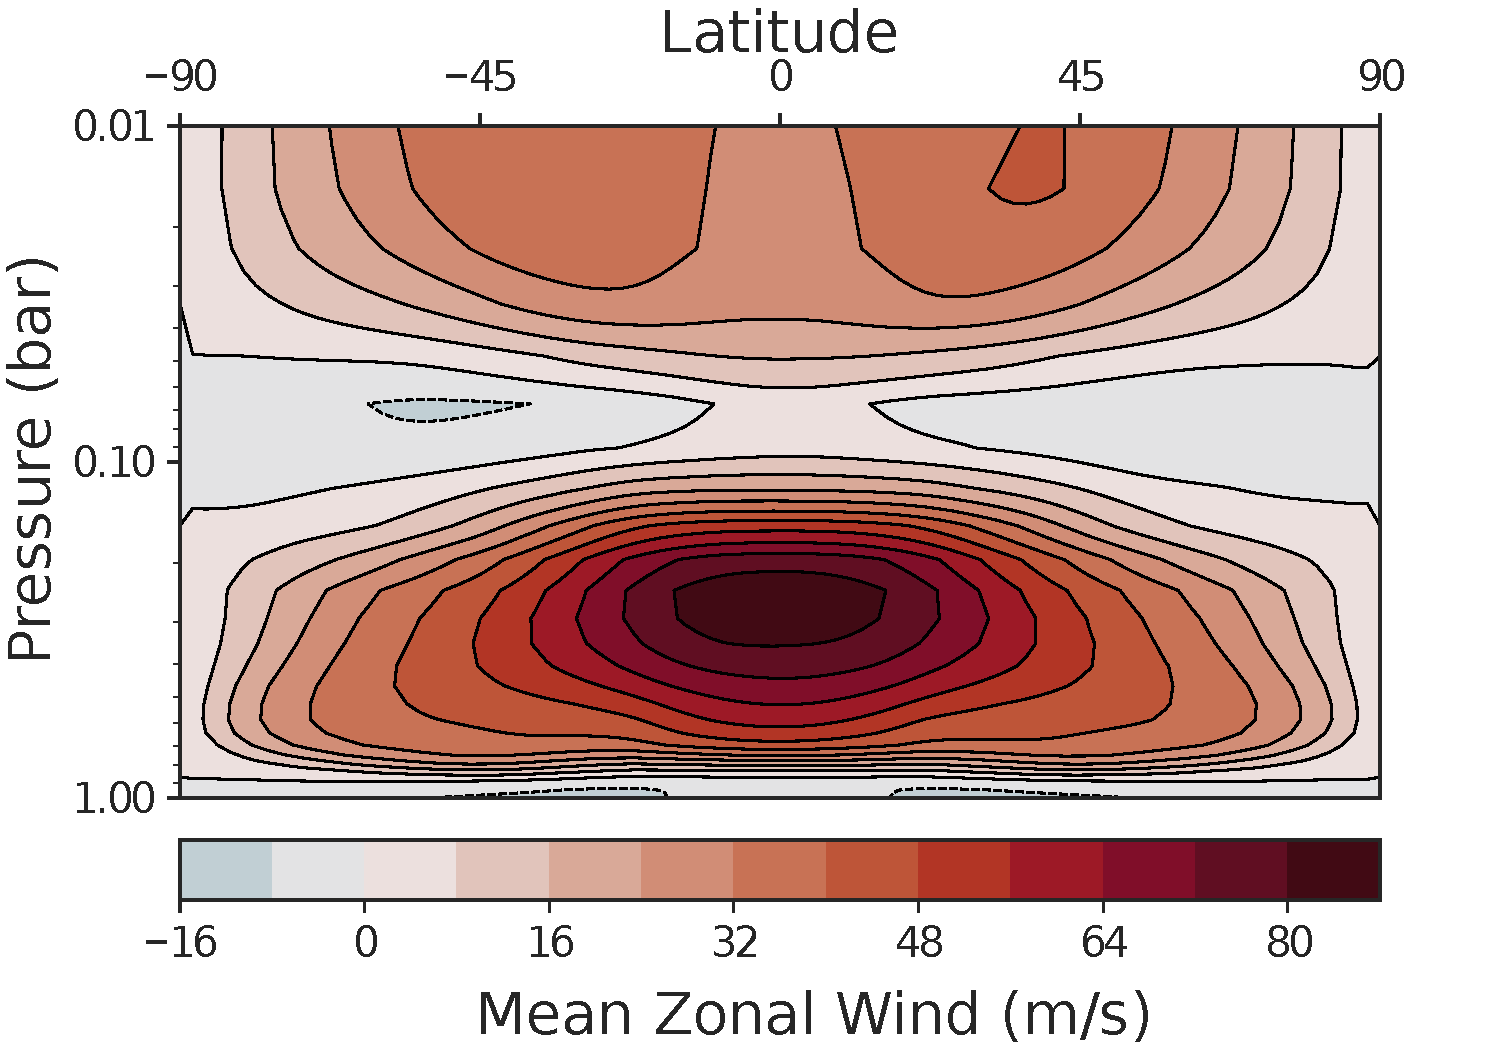
\includegraphics[width=\textwidth]{figures/eqm-zonal-flow/wind-hot-10.pdf}
    \caption{Hot, 10 days}
  \end{subfigure}
  \begin{subfigure}[b]{0.32\textwidth}
    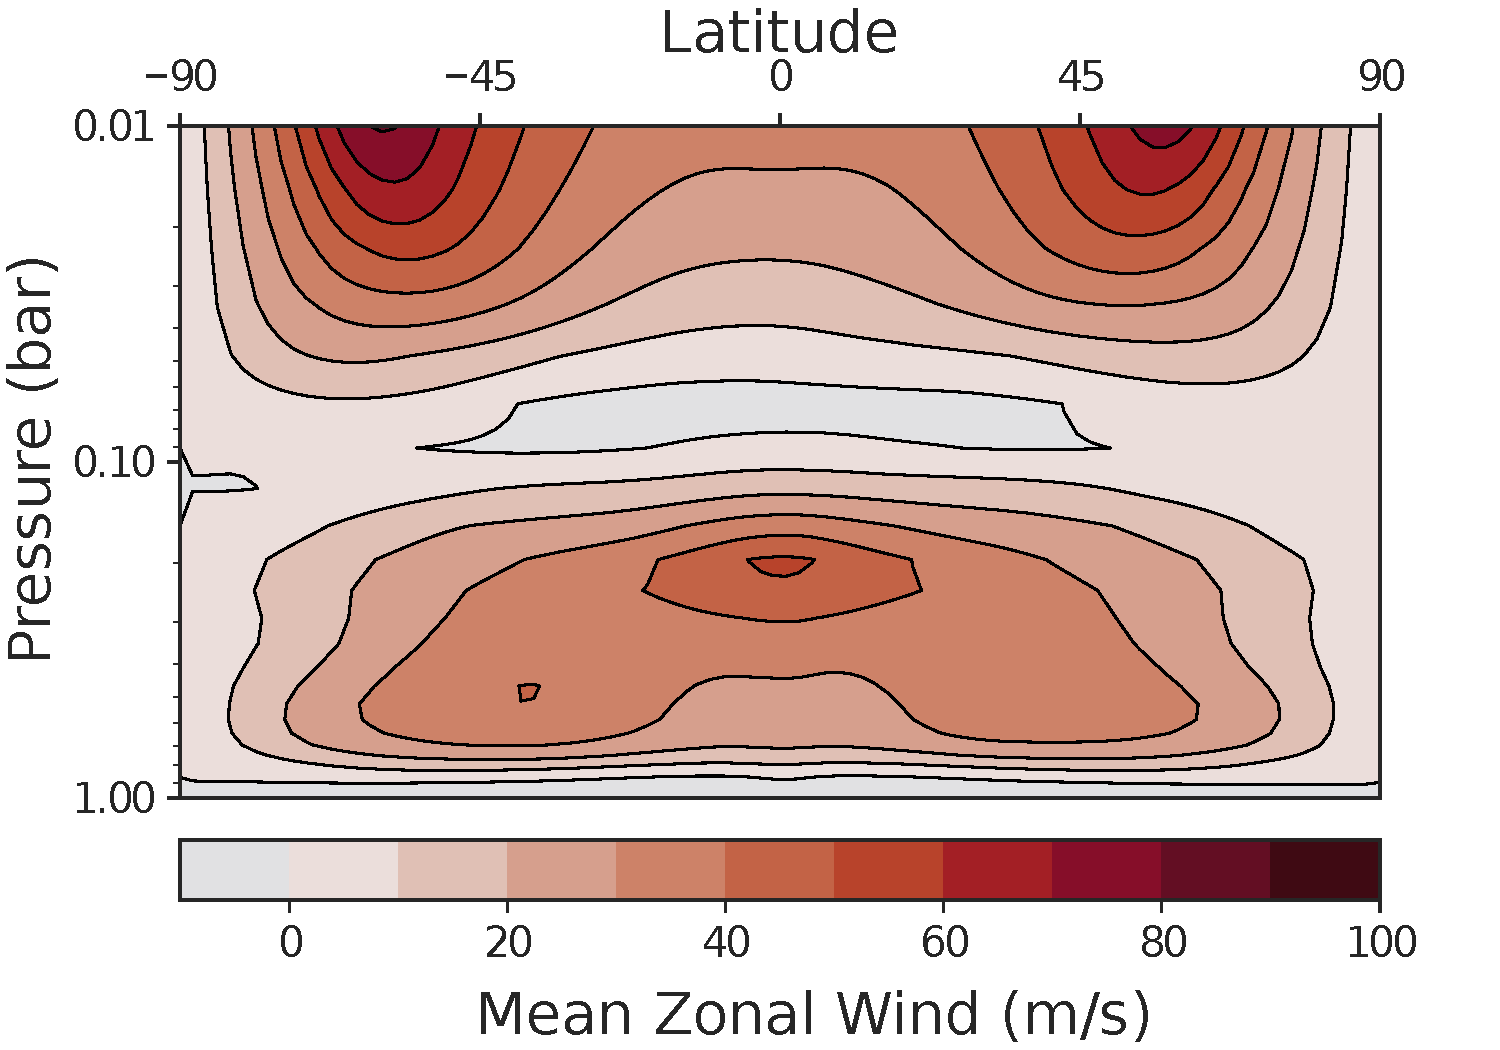
\includegraphics[width=\textwidth]{figures/eqm-zonal-flow/wind-med-10.pdf}
    \caption{Medium, 10 days}
  \end{subfigure}
  \begin{subfigure}[b]{0.32\textwidth}
    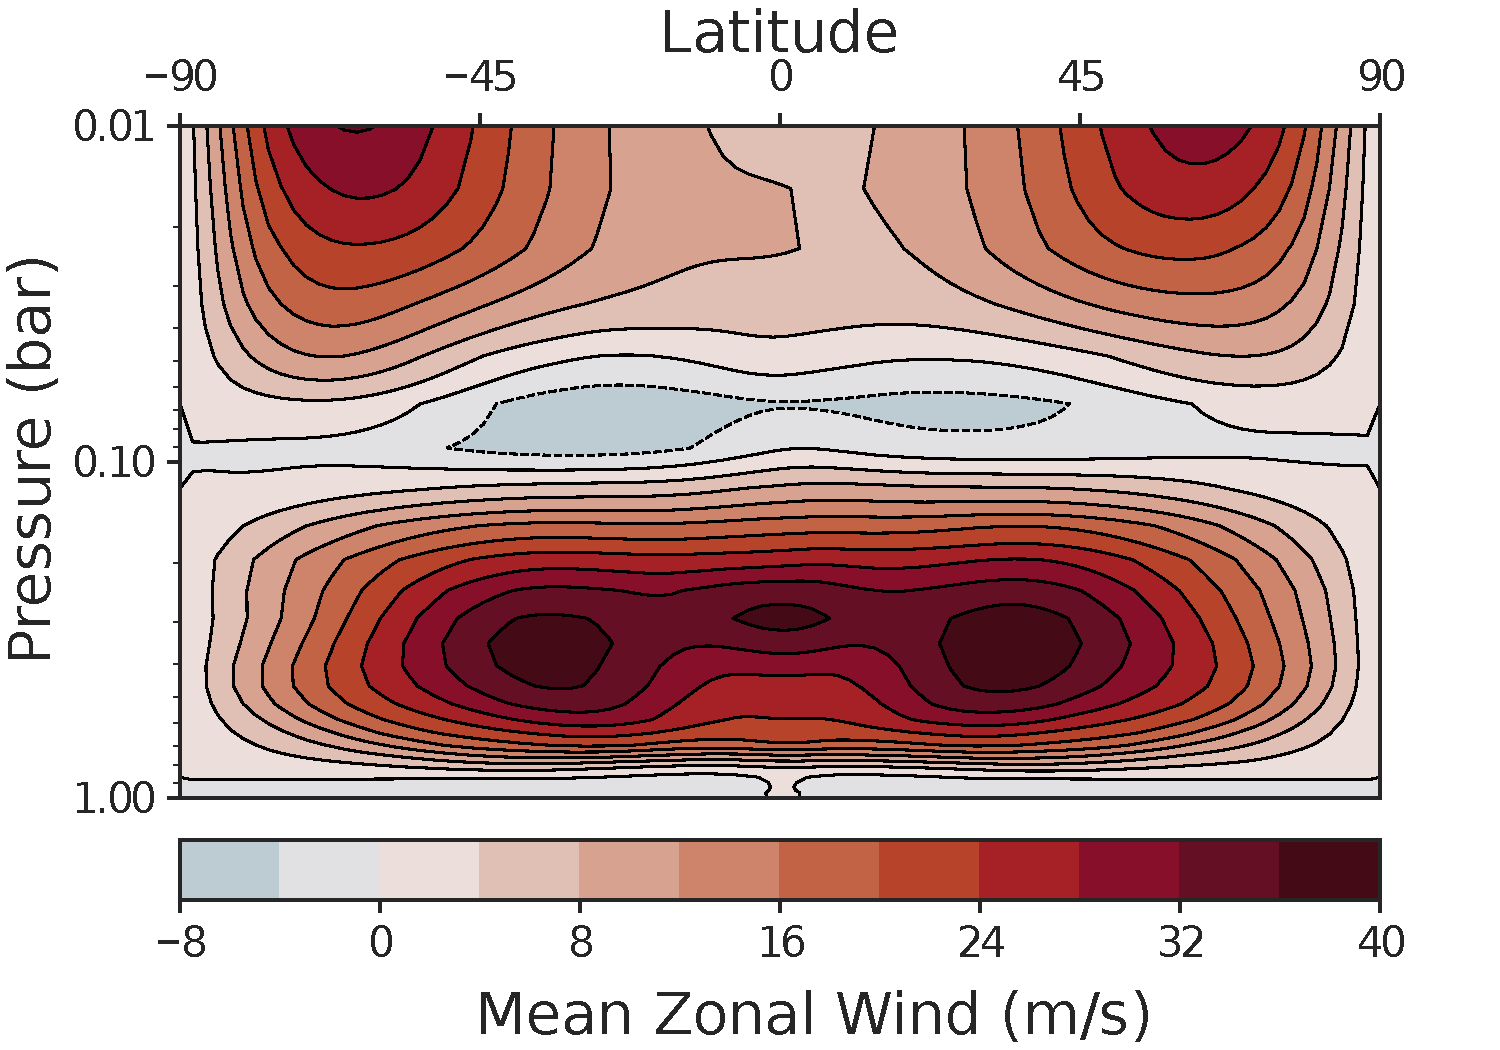
\includegraphics[width=\textwidth]{figures/eqm-zonal-flow/wind-cold-10.pdf}
    \caption{Cold, 10 days}
  \end{subfigure}
    \\
    \begin{subfigure}[b]{0.32\textwidth}
      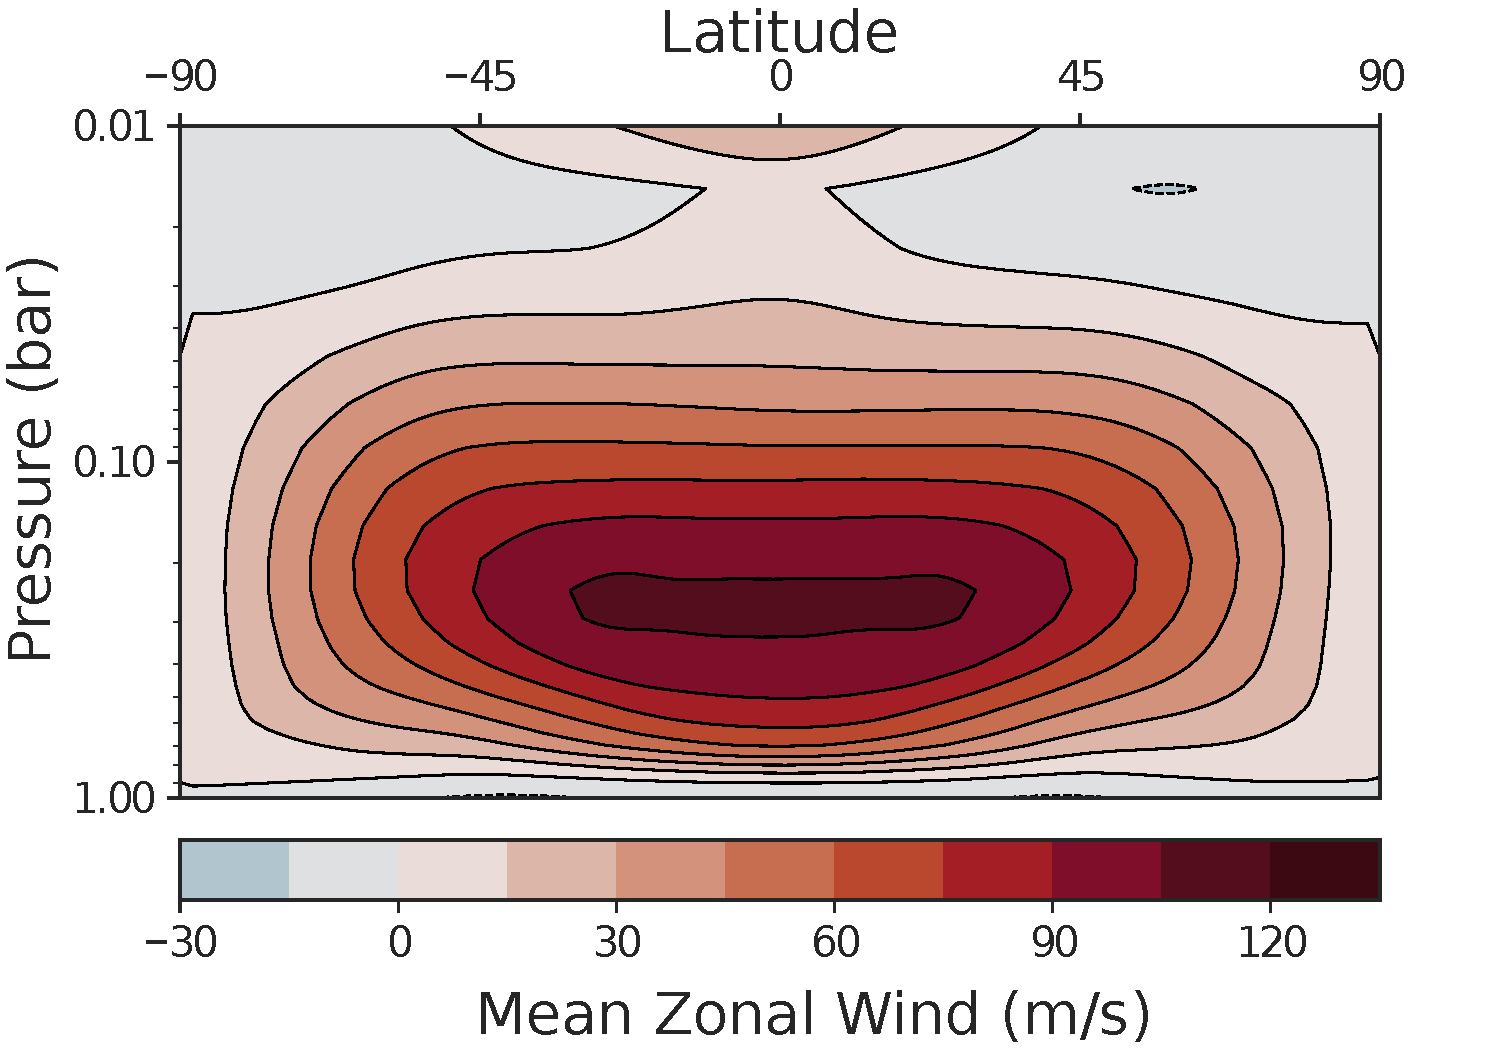
\includegraphics[width=\textwidth]{figures/eqm-zonal-flow/wind-hot-5.pdf}
      \caption{Hot, 5 days}
    \end{subfigure}
    \begin{subfigure}[b]{0.32\textwidth}
      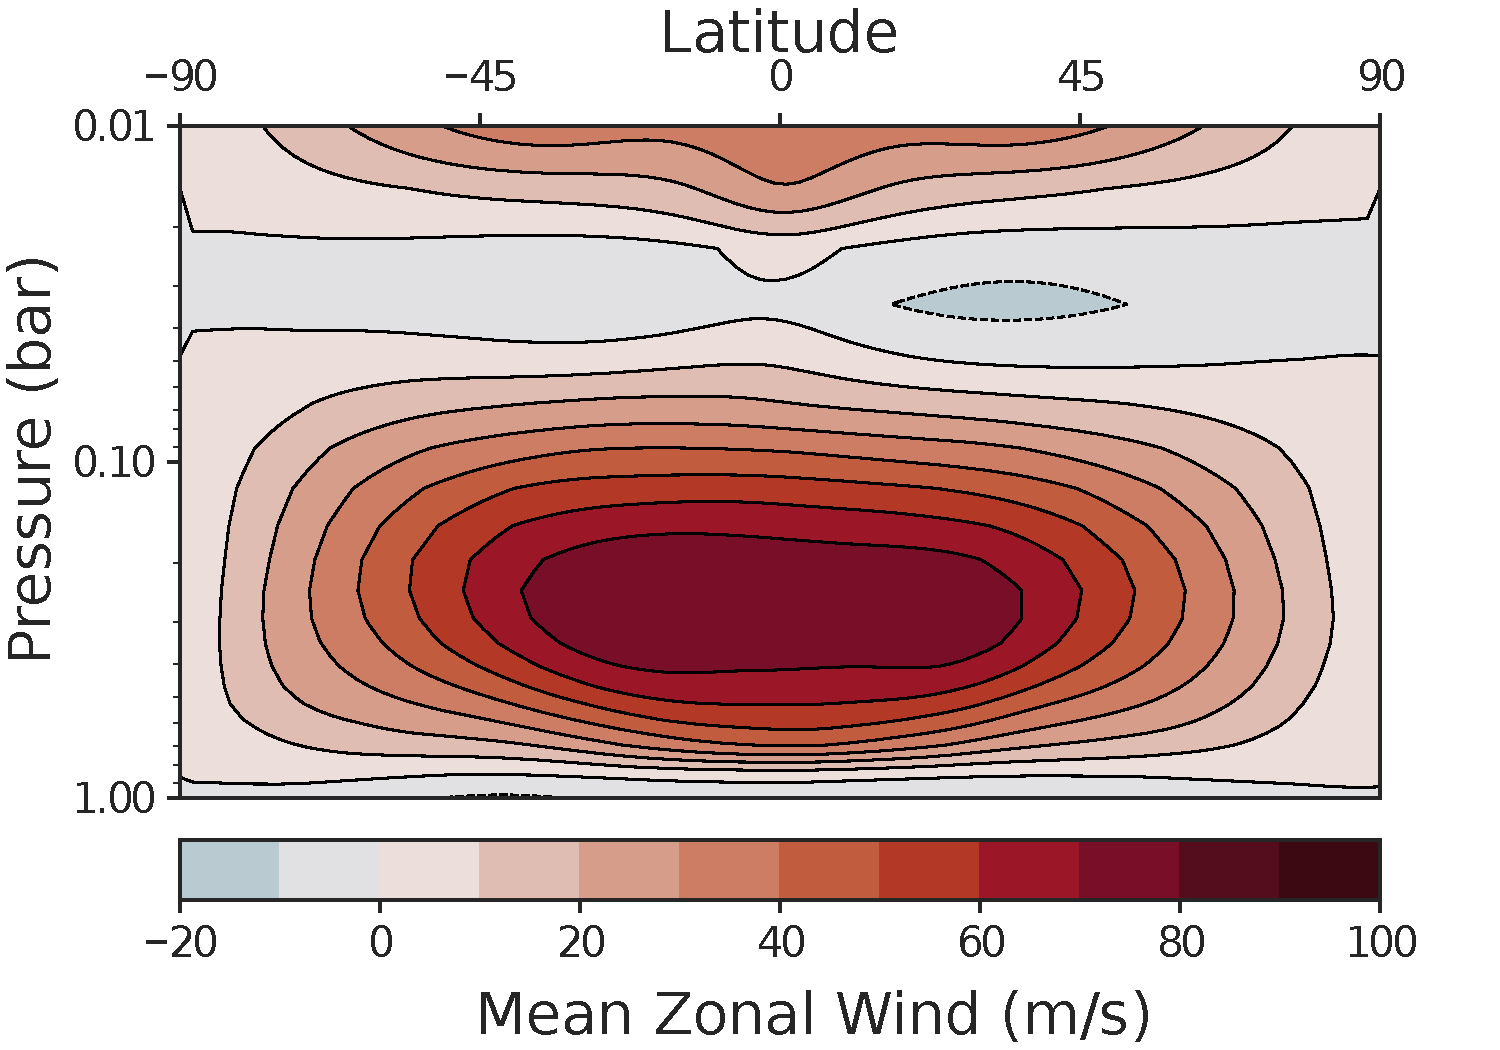
\includegraphics[width=\textwidth]{figures/eqm-zonal-flow/wind-med-5.pdf}
      \caption{Medium, 5 days}
    \end{subfigure}
    \begin{subfigure}[b]{0.32\textwidth}
      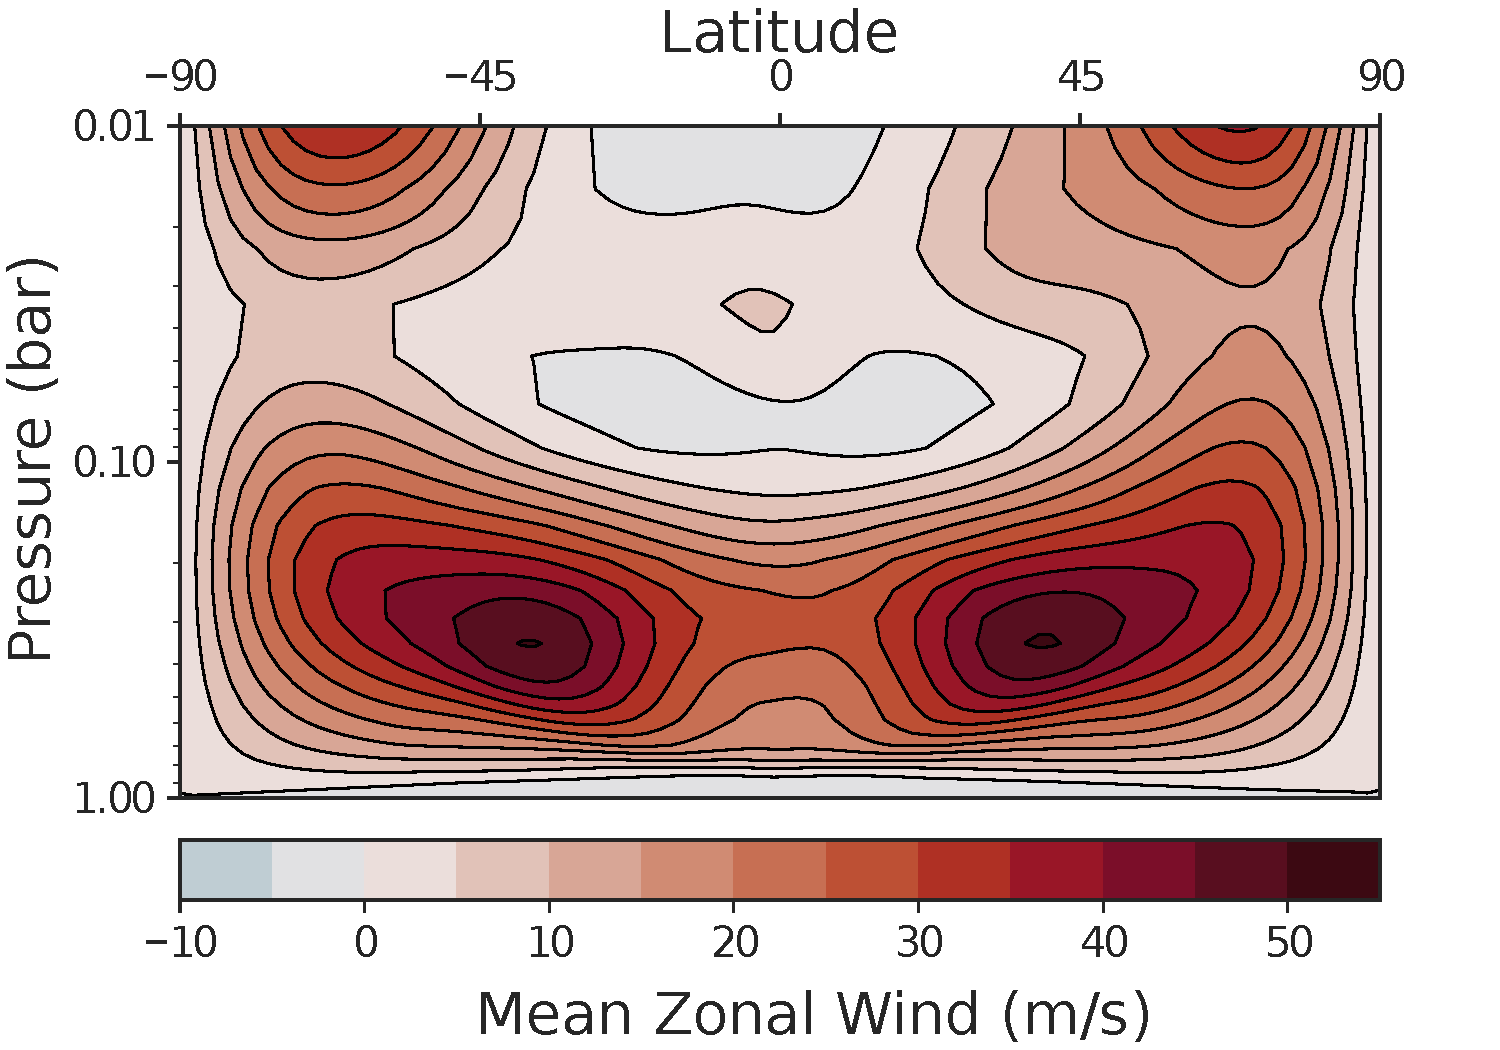
\includegraphics[width=\textwidth]{figures/eqm-zonal-flow/wind-cold-5.pdf}
      \caption{Cold, 5 days}
    \end{subfigure}
     \\
     \begin{subfigure}[b]{0.32\textwidth}
       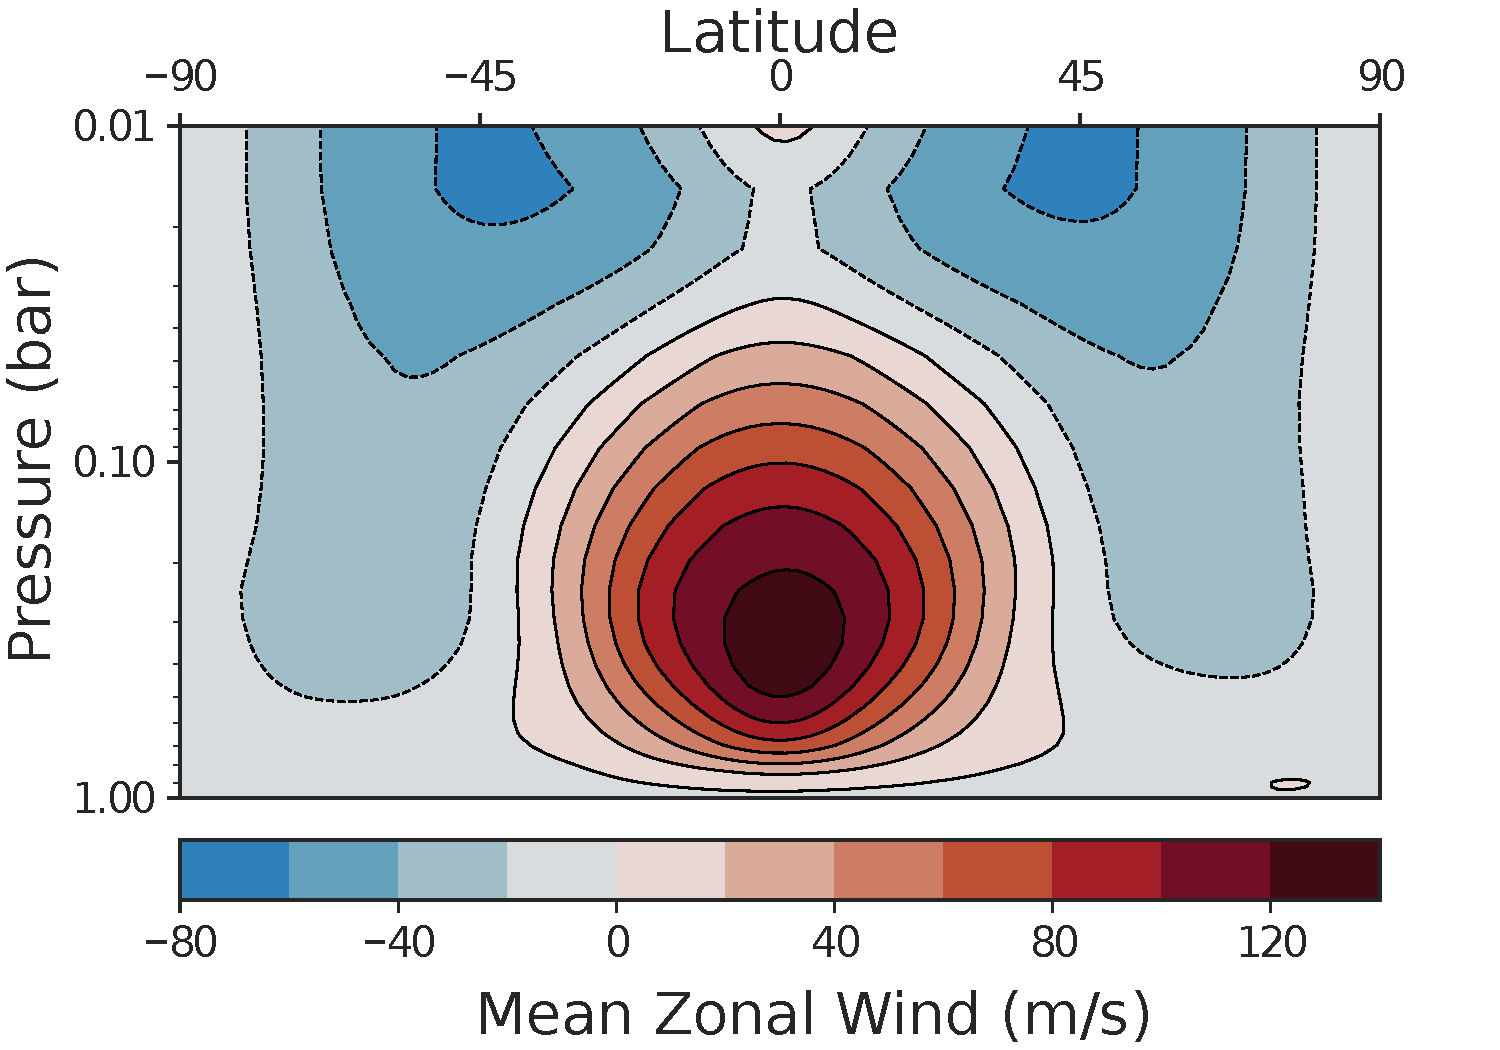
\includegraphics[width=\textwidth]{figures/eqm-zonal-flow/wind-hot-2.pdf}
       \caption{Hot, 2 days}
     \end{subfigure}
     \begin{subfigure}[b]{0.32\textwidth}
       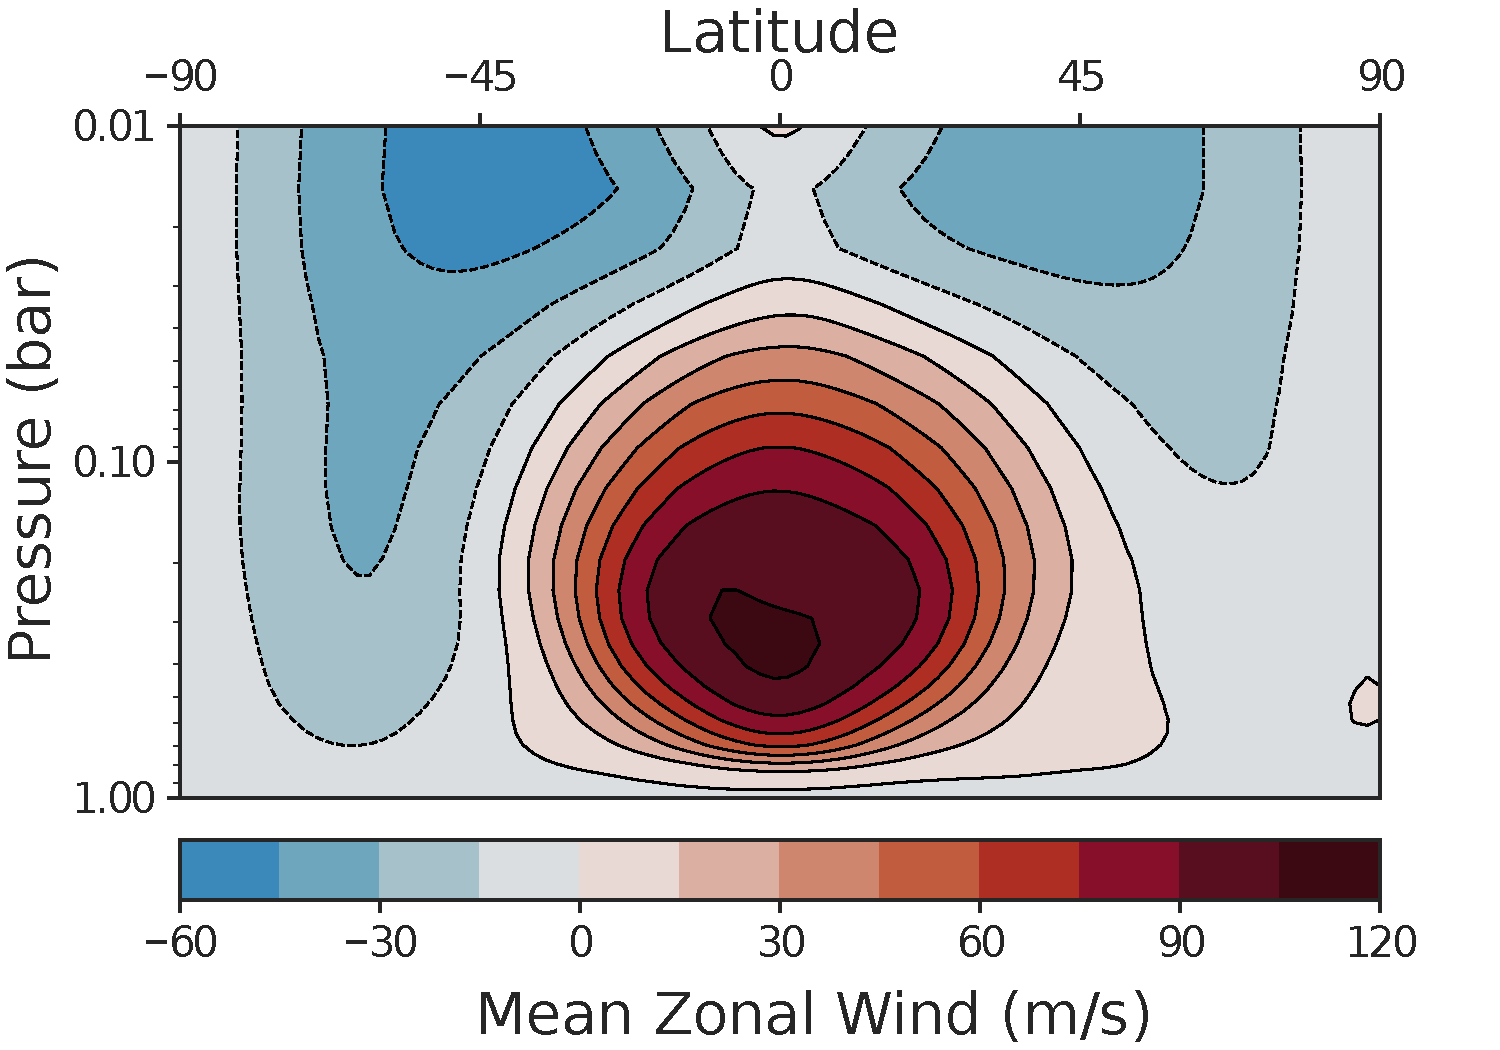
\includegraphics[width=\textwidth]{figures/eqm-zonal-flow/wind-med-2.pdf}
       \caption{Medium, 2 days}
     \end{subfigure}
     \begin{subfigure}[b]{0.32\textwidth}
       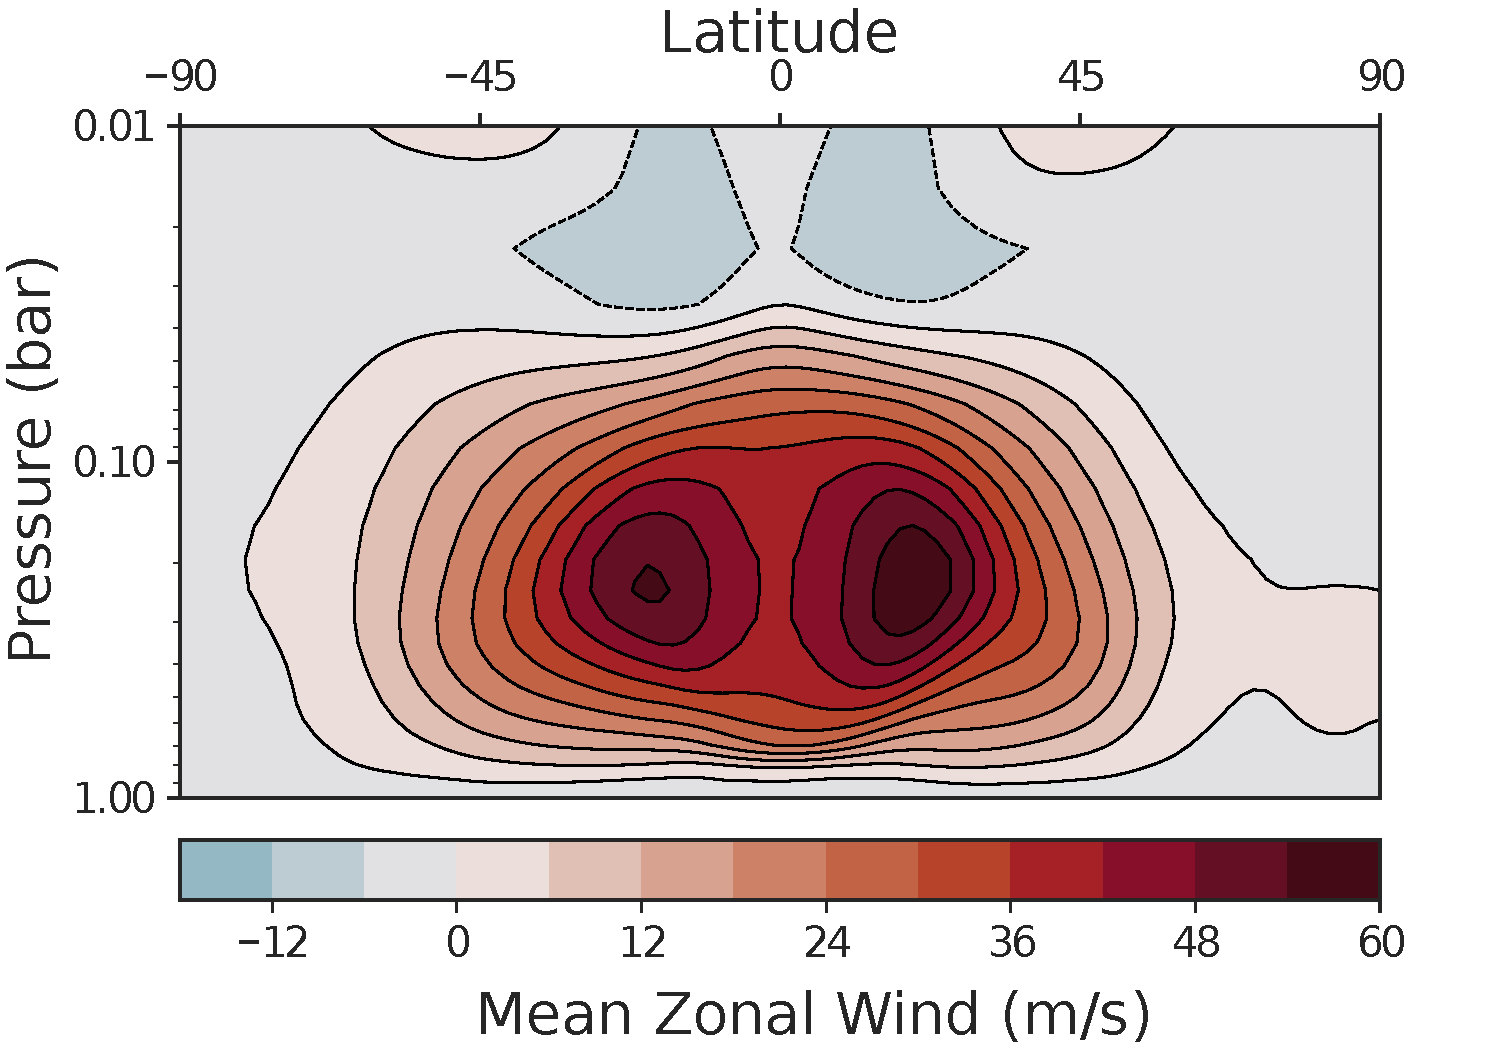
\includegraphics[width=\textwidth]{figures/eqm-zonal-flow/wind-cold-2.pdf}
       \caption{Cold, 2 days}
     \end{subfigure}
  \caption{Scaling \citep{pierrehumbert2018review}.}
  \label{fig:gcm-suite-jets}
\end{figure}

%%%%%%%%%%%%%%%%%%%%%%%%%%%%%%%%%%%%
%SECTION X -- SCALING RELATIONS
\section{Other Jet Patterns}

The suite of tests in Chapter XX show that the zonal mean wind profile on a tidally locked planet is not always well represented by a Gaussian. There can be only two jets in the midlatitudes, or three jets, one on the equator.

In this section I find the forced response with different jet profiles, and show that the result is not particularly different to the Gaussian jet used up to this point.

Two Jets:

Three Jets:

One Prograde, Two Retrograde:

One Retrograde, two prograde (eddy-driven):



%%%%%%%%%%%%%%%%%%%%%%%%%%%%%%%%%%%%
%CONCLUSION
\section{Conclusion}


%RESTATE SECTION CONCLUSIONS

%OPEN OUT CONCLUSIONS






% \bibliographystyle{unsrtnat}
% \bibliography{../references.bib}
